\documentclass{hotnets19}

\usepackage{times}  
\usepackage{hyperref}
\usepackage{listings, multicol}
\usepackage{lipsum}
\usepackage{xcolor}
\usepackage{graphicx}
\usepackage{subcaption}
\usepackage{mdframed}


\usepackage{float}
% \usepackage[export]{adjustbox}

\usepackage{booktabs}

\hypersetup{pdfstartview=FitH,pdfpagelayout=SinglePage}

\setlength\paperheight {11in}
\setlength\paperwidth {8.5in}
\setlength{\textwidth}{7in}
\setlength{\textheight}{9.25in}
\setlength{\oddsidemargin}{-.25in}
\setlength{\evensidemargin}{-.25in}


\definecolor{mygray}{gray}{1.0}
\definecolor{commentcolor}{RGB}{0,100,0}
\definecolor{myk}{rgb}{0.0,0,0.65}


\lstdefinelanguage{P4}{
  keywords={in, out, struct, inout, function, return, switch, enum, if, else, case, break, extern, void, bit, error, int, verify, bool, key, table, action, actions, parser, control, state, transition, select, apply},
  keywordstyle=\color{myk}\bfseries,
  keywords=[2]{boolean, string, number, objectid},
  keywordstyle=[2]\color{green}\bfseries,
  identifierstyle=\color{darkgray}\bfseries,
  sensitive=false,
  comment=[l]{//},
  morecomment=[s]{/*}{*/},
  commentstyle=\color{commentcolor}\ttfamily,
  stringstyle=\color{red}\ttfamily,
  morestring=[b]',
  morestring=[b]"
}

\lstset{
   language=P4,
%    numbers=left,
%    backgroundcolor=\color{mygray},
   extendedchars=true,
   basicstyle=\small\ttfamily\color{darkgray}\bfseries,
   showstringspaces=false,
   showspaces=false,
   tabsize=2,
   frame=single,
   breaklines=true,
   showtabs=false
}

\newcommand{\hs}[1]{{\color{blue}{HS:#1}}}

\begin{document}

% \conferenceinfo{HotNets 2019} {}
% \CopyrightYear{2019}
% \crdata{X}
% \date{}

%%%%%%%%%%%% THIS IS WHERE WE PUT IN THE TITLE AND AUTHORS %%%%%%%%%%%%

\title{MicroP4}

\author{Paper \#0, 3 pages}

\maketitle

%%%%%%%%%%%%%  ABSTRACT GOES HERE %%%%%%%%%%%%%%
\begin{abstract}
Domain-specific languages such as P4 enable flexible and efficient
packet-processing using primitives such as programmable parsers and
re-configurable match-action tables. However, the P4 ecosystem exposes
details of the underlying architecture, which ties programs to
specific architectures and makes it difficult to write composeable
libraries of code that can be reused across many different programs.

To address this challenge, we present the design and implementation of
a logical target, MicroP4 ($\mu$P4), that decouples P4 programs from
architecture-specific constructs and naturally supports composition.
We present the design of the $\mu$P4 architecture ($\mu$SA), which
abstracts away from hardware-level details without sacrificing
expressiveness. Using realistic examples, we show how $\mu$P4 enables
modular programming, and we present a prototype implementation of the
$\mu$P4C compiler that generates code for lower-level architectures
such as PISA, which is implemented by the Bmv2 software switch.
\end{abstract}

\section{Introduction}

% hardware and software together, cool
Over the last decade, the synergistic development of packet-processing
hardware and software has fundamentally changed how networks are built
and operated. Hardware platforms such as
RMT~\cite{Bosshart:2013:FMF:2486001.2486011} provide tremendous
flexibility for customizing the forwarding plane without having to
fabricate new chips, while languages such as
P4~\cite{Bosshart:2014:PPP:2656877.2656890, p4lang} enable programmers
to describe rich packet-processing functions in terms of high-level
abstractions such as parsers and match-action tables.

In order to support different kinds of targets (e.g., software
switches, ASICs, FPGAs, etc.), P4 allows programmable and
fixed-function blocks to be arranged into different layouts as
specified by an architecture declaration. For example, the Protocol
Independent Switch Architecture
(PISA)~\cite{Bosshart:2013:FMF:2486001.2486011} models a switch with a
programmable parser, programmable ingress pipeline, fixed-function
scheduler and queues, programmable egress pipeline, and programmable
deparser. PISA programs supply P4 code for each programmable block.
But while this design allows the language to flexibly accommodate a
wide range of targets, it also creates a tight coupling between
programs and architectures, which makes it difficult to write programs
in a compositional manner or reuse common code fragments in different
programs.

For example, \texttt{switch.p4}~\cite{switch.p4} handles several dozen
different protocols and functions (e.g., L2 switching, L3 routing,
tunneling, etc.,). But the code is written against a global collection
of q metadata and parsed headers. To use the code in
\texttt{switch.p4} to implement an Ethernet switch, it would be
necessary to detangle the L2-specific functionality from the
extraneous code in the rest of the program. Without a detailed
understanding of the overall structure of the top-level program, it is
difficult or impossible to reuse code fragments at finer granularity.

% \section{Use Case}
Consider a simple scenario, as shown in Figure~\ref{fig:l3.p4.l2.p4}.
The first program, \texttt{l3.p4}, parses the IPv4 header, uses
longest-prefix matching to determine the next hop, decrements the
\texttt{ttl} field and, finally, deparses the packet. The second
program, \texttt{l2.p4}, parses the Ethernet header, and modifies the
ethernet addresses using the next hop, which is supplied as an
argument, and finally deparses the packet. Note that neither
\texttt{l3.p4} nor \texttt{l2.p4} is a complete packet-processing
program: the former does not generate a functionally correct packets,
while the latter is parameterized on the next hop and so does not
specify forwarding behavior. However, we could combine \texttt{l2.p4}
with any other routing scheme (e.g., IPv6, MPLS, etc.) to obtain a
valid program. 

\begin{figure*}[ht]
\noindent \begin{minipage}[t]{.48\textwidth}
\begin{lstlisting}[frame=none]
// l3.p4
parser P(packet_in pin, out hdr_t hdrs) {
  state start {
    pin.extract(hdrs.eth);
    transition select(hdrs.eth.ethType){
       0x0800: parse_ipv4;
    }
  }
  state parse_ipv4 {
      pin.extract(hdrs.ipv4);
      transition accept;
  }
}
control Pipe(inout hdr_t hdrs, out bit<16> nexthop_id, inout sm_t sm) {
  action process(bit<16> nh) {
    hdrs.ipv4.ttl = hdrs.ipv4 - 1;
    nexthop_id = nh;// setting out param
  }
  table ipv4_lpm_tbl {
    key = { hdrs.ipv4.dstAddr : lpm } 
    actions = { process; }
  }
  apply { ipv4_lpm_tbl.apply(); }
}
control D(packet_out po, in hdr_t hdrs) {
  apply { po.emit(hdrs.eth); po.emit(hdrs.ipv4); }
}
\end{lstlisting}
\end{minipage}
\hfill\begin{minipage}[t]{.48\textwidth}
\begin{lstlisting}[frame=none]
// l2.p4
parser P(packet_in pin, out hdr_t hdrs) {
  state start {
    pin.extract(hdrs.eth);
  }
}
control Pipe(inout hdr_t hdrs, inout sm_t sm, 
             in bit<16> nexthop_id) {
  action drop () {}           
  action forward(bit<48> dest_mac, 
                 bit<48> src_mac, bit<8> port) {
    hdrs.eth.dstAddr = dest_mac;
    hdrs.eth.srcAddr = src_mac;
    sm.out_port = port;    
  }
  table forward_tbl {
    key = { nexthop_id : exact; } 
    actions = { process; drop; }
  }
  apply {
    forward_tbl.apply(); 
    if (sm.deq_qdepth > 100) // rate limiting
      drop();
  }
}
control D(packet_out po, in hdr_t hdrs) {
  apply { po.emit(hdrs.eth); }
}
\end{lstlisting}
\end{minipage}
% \vspace*{-10pt}
\caption{Example: \texttt{l3.p4} and \texttt{l2.p4}.}
\label{fig:l3.p4.l2.p4}
\end{figure*}


%% The current ecosystem of programmable data plane enforces programmers
%% to write code amenable to the target device's data plane architecture
%% and pipeline. Programmers write code for programmable blocks taking
%% into account their location in pipeline rather than compilers
%% automatically allocating code to the appropriate blocks. We believe
%% that devices should only expose abstraction for processing blocks and
%% the onus of code allocation to the blocks in pipeline should be on
%% compilers for the devices.

There is some prior work on modular composition of P4 programs.
Systems such as HyPer4 \cite{Hancock:2016:HUP:2999572.2999607},
HyperV~\cite{8038396}, and
P4Visor~\cite{Zheng:2018:PLV:3281411.3281436} provide constructs for
merging independent programs onto a single device. However, these
systems only handle programs that describe end-to-end
packet-processing functions. Hence, they lack mechanisms for enabling
selective reuse of library code, specifying interfaces between
modules, and facilitating inter-module communication. To write truly
modular P4 programs, a fundamentally different approach is needed.

To this end, this paper presents the design and (prototype)
implementation of $\mu$P4, a new architecture that provides
fine-grained abstractions for constructing data plane programs.
$\mu$P4 consists of two components, Micro Switch Architecture
($\mu$SA), which distills packet processing to its essence, and
abstracts away from device-specific structure, and a compiler,
$\mu$P4C, that maps one or more $\mu$SA programs to a standard PISA
pipeline. 

This paper makes the following contributions.
\begin{itemize}
\item We motivate the need for modular data plane programming using a
  series of realistic examples.
\item We introduce $\mu$ SA, a new P4 architecture designed to enable
  fine-grained composition of program snippets.
\item We develop techniques for compiling $\mu$SA programs to the
  standard PISA model, including merging programs composed together in
  parallel or in sequence onto a single PISA pipeline.
\end{itemize}

Although much work remains, we believe that $\mu$ SA represents a
promising first step toward enabling modular data plane programs.

\section{Challenges}
P4 is developed to specify data plane functionality of software or hardware targets (e.g., simple\_\-switch \cite{simple_switch.md}, TOFINO \cite{tofino} etc.,) devices.
Target device manufacturer provides an architecture description of data plane along with a P4 compiler for the device.
The architecture source file (e.g., v1\-mod\-el\-.p4 \cite{v1model.p4} for simple\_switch) contains declaration of a set of pro\-gram\-ma\-ble blocks, their data plane interfaces and the target specific metadata (called intrinsic metadata) and extern functions.
To program the packet processing pipeline of a device, P4 programmers provide implementation of the declared programmable blocks in its architecture file.
Therefore, P4 programs are tightly coupled with architecture of the target devices.

\begin{figure}[H]
    \begin{subfigure}[b]{\linewidth}
        \centering
        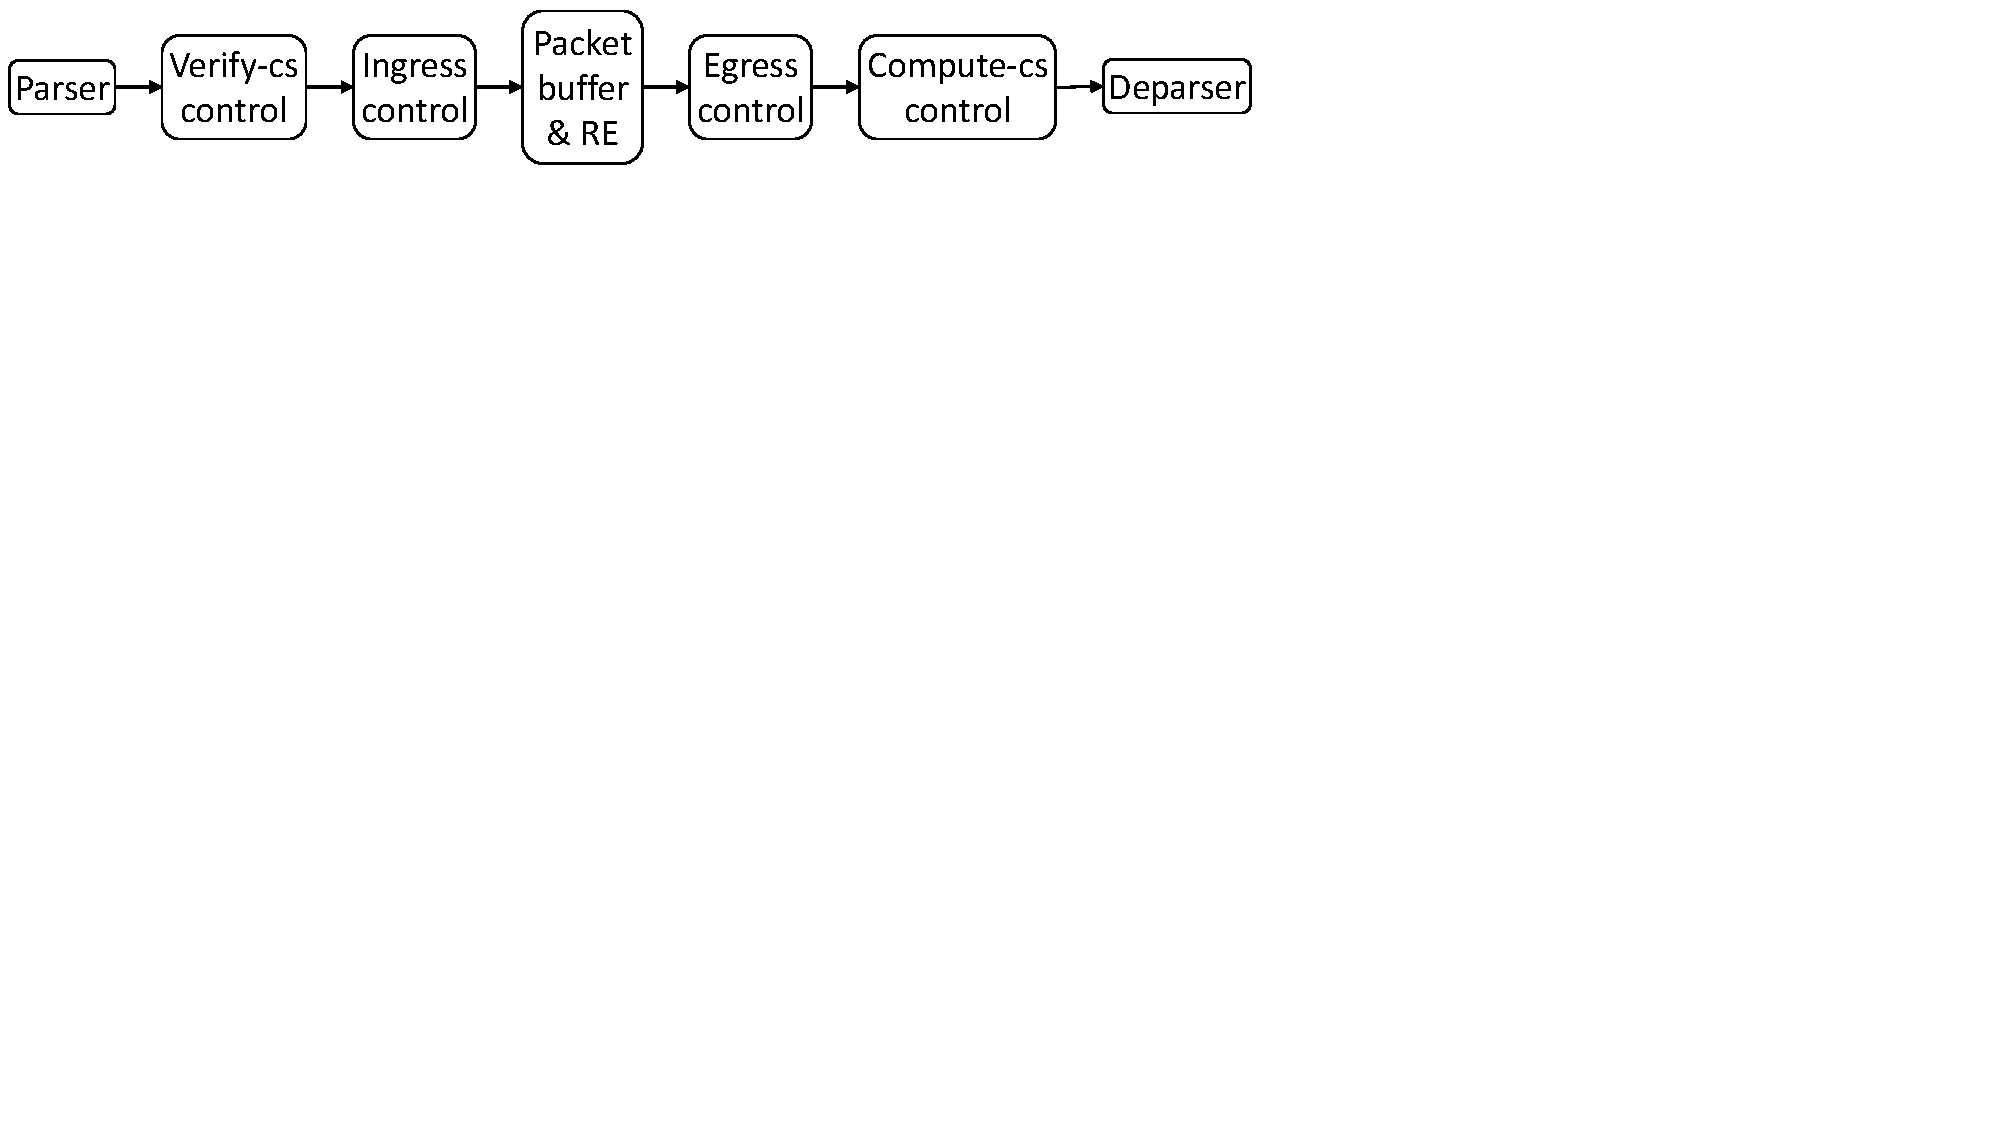
\includegraphics[trim=2 460 380 0, clip,scale=0.37]{v1model-pipeline.pdf}
        \caption{simple\_switch v1 Model}
        \label{subfig:v1model}
    \end{subfigure}
    \begin{subfigure}{\linewidth}
        \centering
        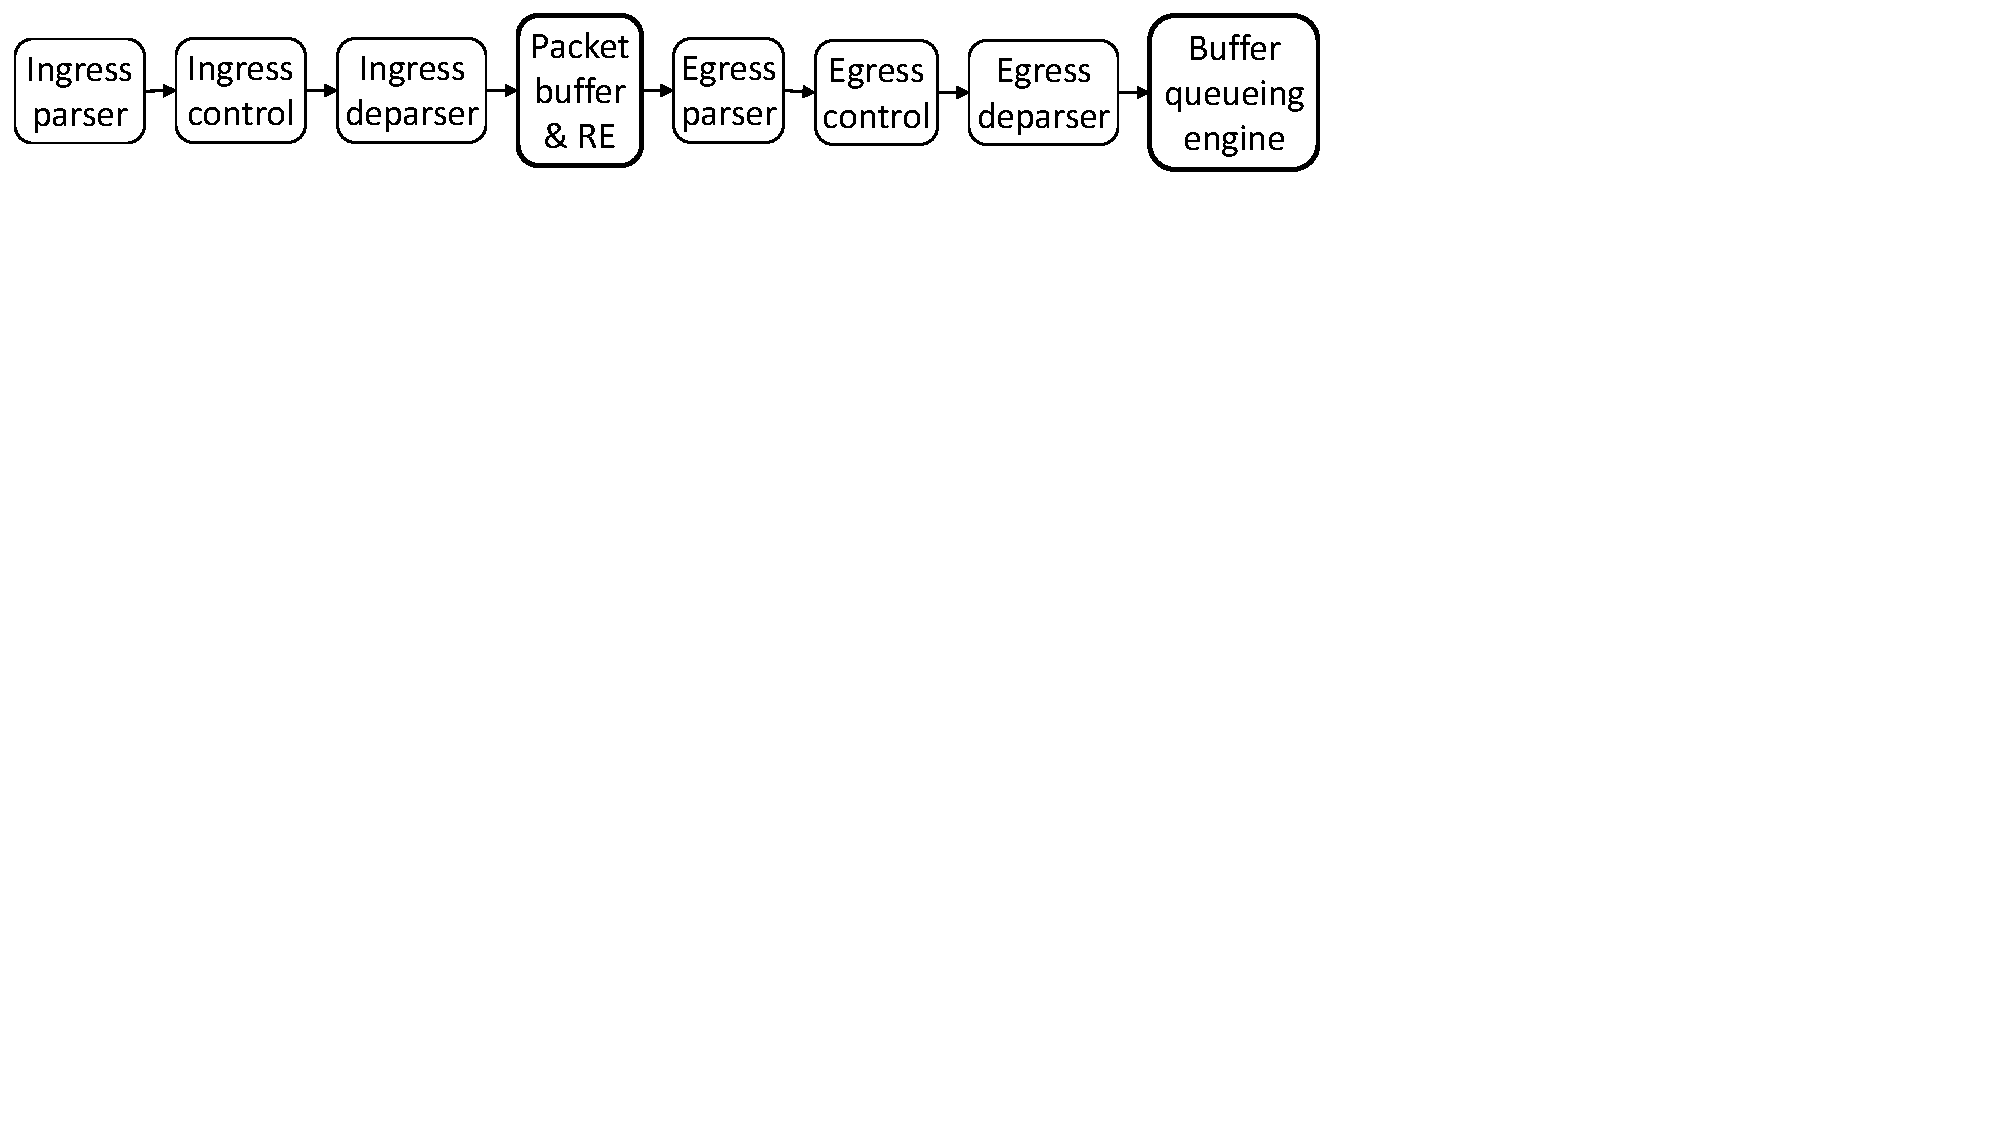
\includegraphics[trim=2 450 281 0, clip,scale=0.37]{psa-pipeline.pdf}
        \caption{PSA Model}
        \label{subfig:psa-model}
    \end{subfigure}
\caption{Real Target Architectures}
\label{fig:real-target-architectures}
\end{figure}

The architecture description of a target specifies data plane pipeline comprising a set of pro\-gram\-ma\-ble and fixed-function blocks, flow of user-defined and target-specific (called intrinsic) metadata in the pipeline and semantics of target-specific actions and externs.
For example, Figure \ref{subfig:psa-model} and \ref{subfig:v1model} show data plane pipelines and their packet processing blocks defined in v1model \cite{simple_switch.md} and Portable Switch Architecture (PSA) \cite{psa}, respectively.


Parser blocks are described using a sub-language of P4, based on abstraction of Finite State Machine.
Control blocks are expressed using a sub-language modelling imperative control flow.
Deparsers are special control blocks that allows to use statements, to reassemble packets, that are prohibited in other control blocks.
Packet processing logic in P4 programs are sectioned across programmable blocks with heterogeneous abstract machines (e.g., parsers, deparsers, control) and fixed-function blocks (Packet Buffer and Replication Engine).
Therefore, a control block can not instantiate and execute parser blocks. Similarly, deparser block can not invoke and execute parser blocks.  
Consider the example in Figure \ref{fig:l3.p4.l2.p4}, parser ``P'' of l2.p4 can not be executed at the end of deparser control block ``D'' of l3.p4.


Moreover, architectures models expose intrinsic metadata, target-specific actions and extern functions (e.g., resubmit, recirculate, clone) to replicate and/or program packet-path and flow of data across the processing blocks, as described in \cite{simple_switch.md} and  \cite{psa}
In turn, adding different abstract-machine to program packet-path and data flow across the blocks and further increasing heterogeneity in the model of a data plane program.
<<For example, resubmit or recirculate calls are like event trigger.. effects happen after the block>>

Finally, the existing architecture models expose target-spe\-cific constraints to programmers.
E.g., output port can not be changed in egress control block, scope of some intrinsic metadata limited to specific programmable blocks, etc.,  
Programmers need implement execution logic conforming to constraints, architecture model and semantics of actions and extern functions of the target device.


% P4 programmers need to implement homogeneous blocks (e.g., ingress and egress control) satisfying different accessibility constraints on intrinsic metadata exposed by the architecture. 

The absence of a uniform abstract machine for packet processing and presence of target-specific constraints have made extremely difficult to enable modularity.
Because, modularity requires mechanisms to develop independent code modules and interface to reuse them without requiring to know their implementation detail.
Also, existing compilers and architecture specifications do not provide simplified and common abstractions for packet processing blocks in data plane to facilitate target agnostic reuse of data plane programs.


% In section \ref{section:micros-awitch-architecture}, we explain the design of Micro Switch Architecture for a logical target that reduces number of programmable blocks and introduces logical externs to minimize heterogeneity in abstract model of P4 programs.



% \begin{figure}
%  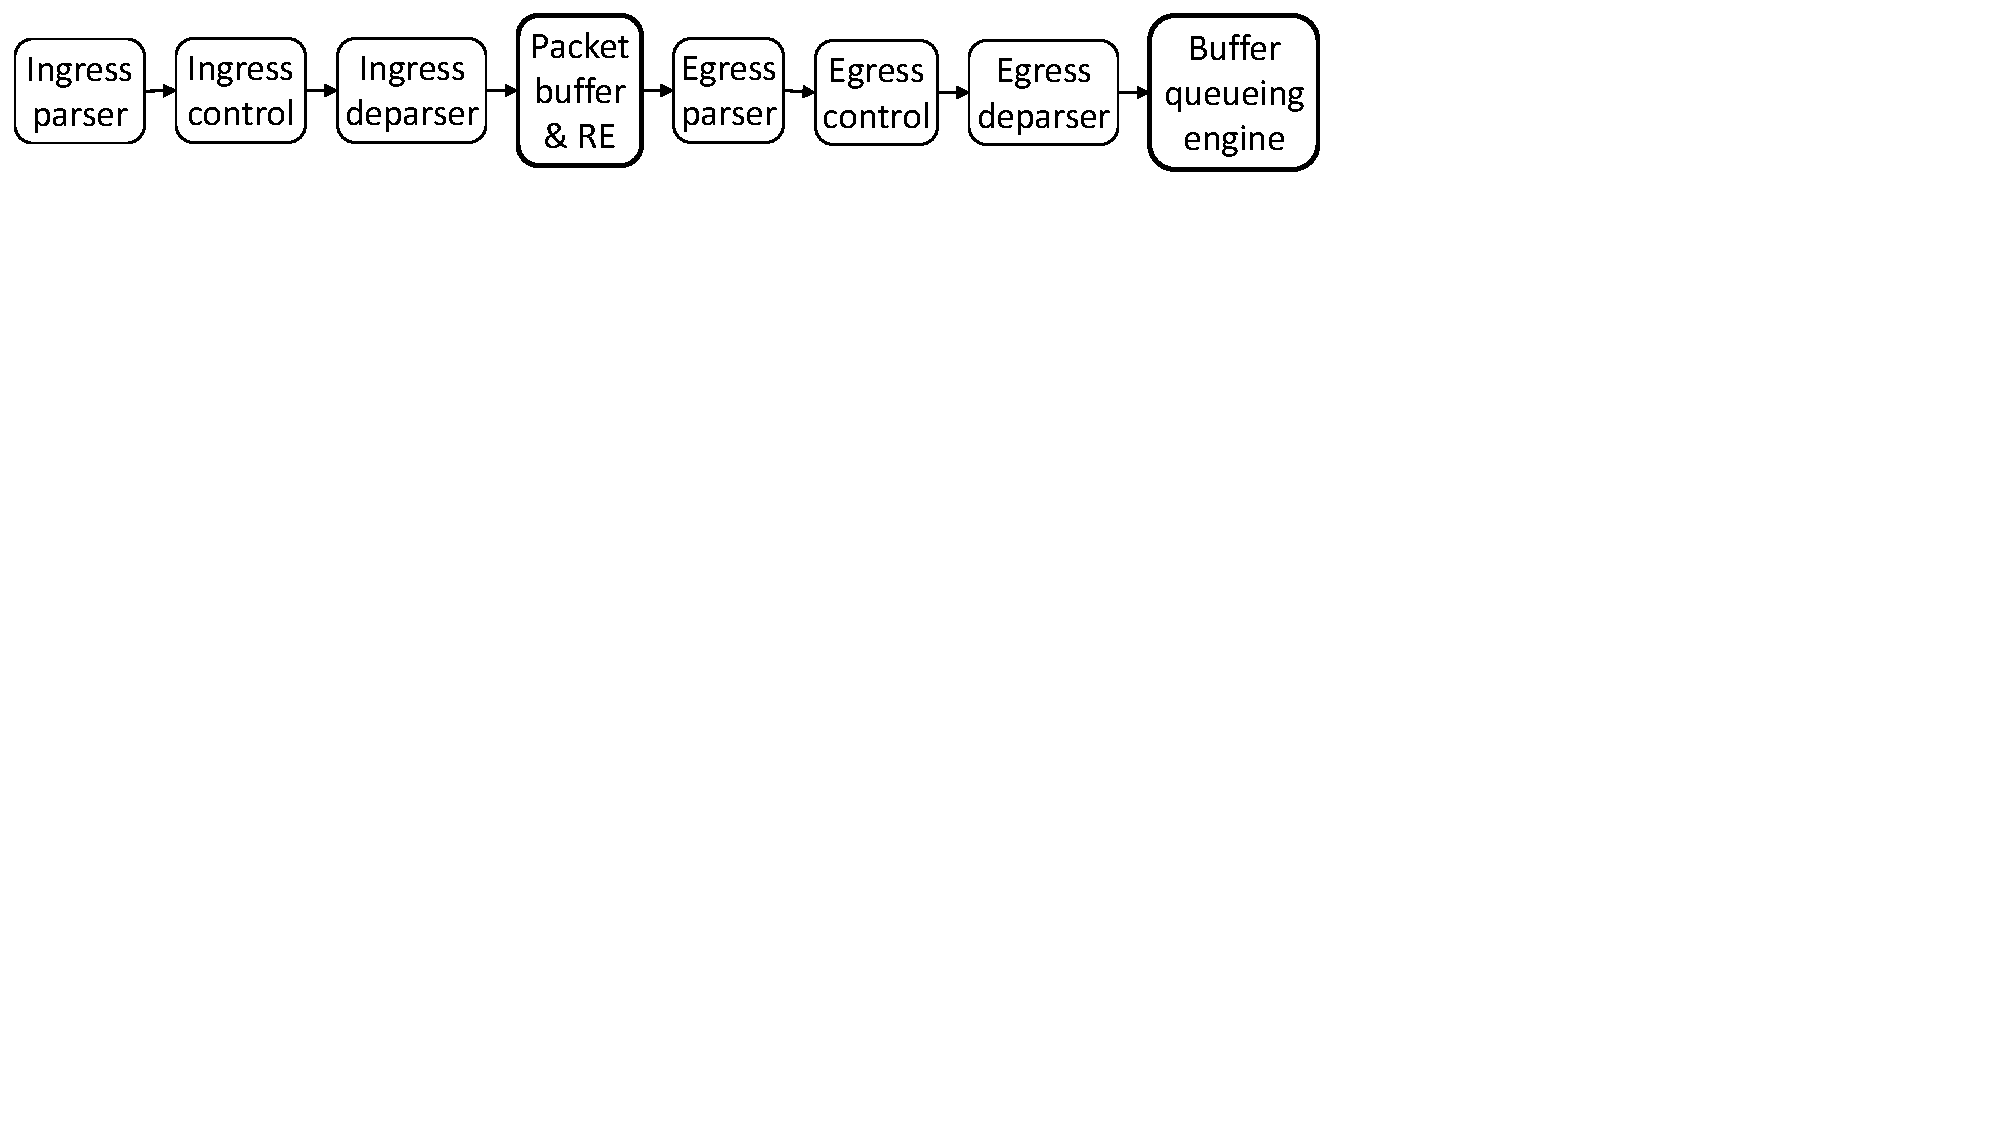
\includegraphics[trim=3 459 281 0, clip,scale=0.35]{psa-pipeline.pdf}
%  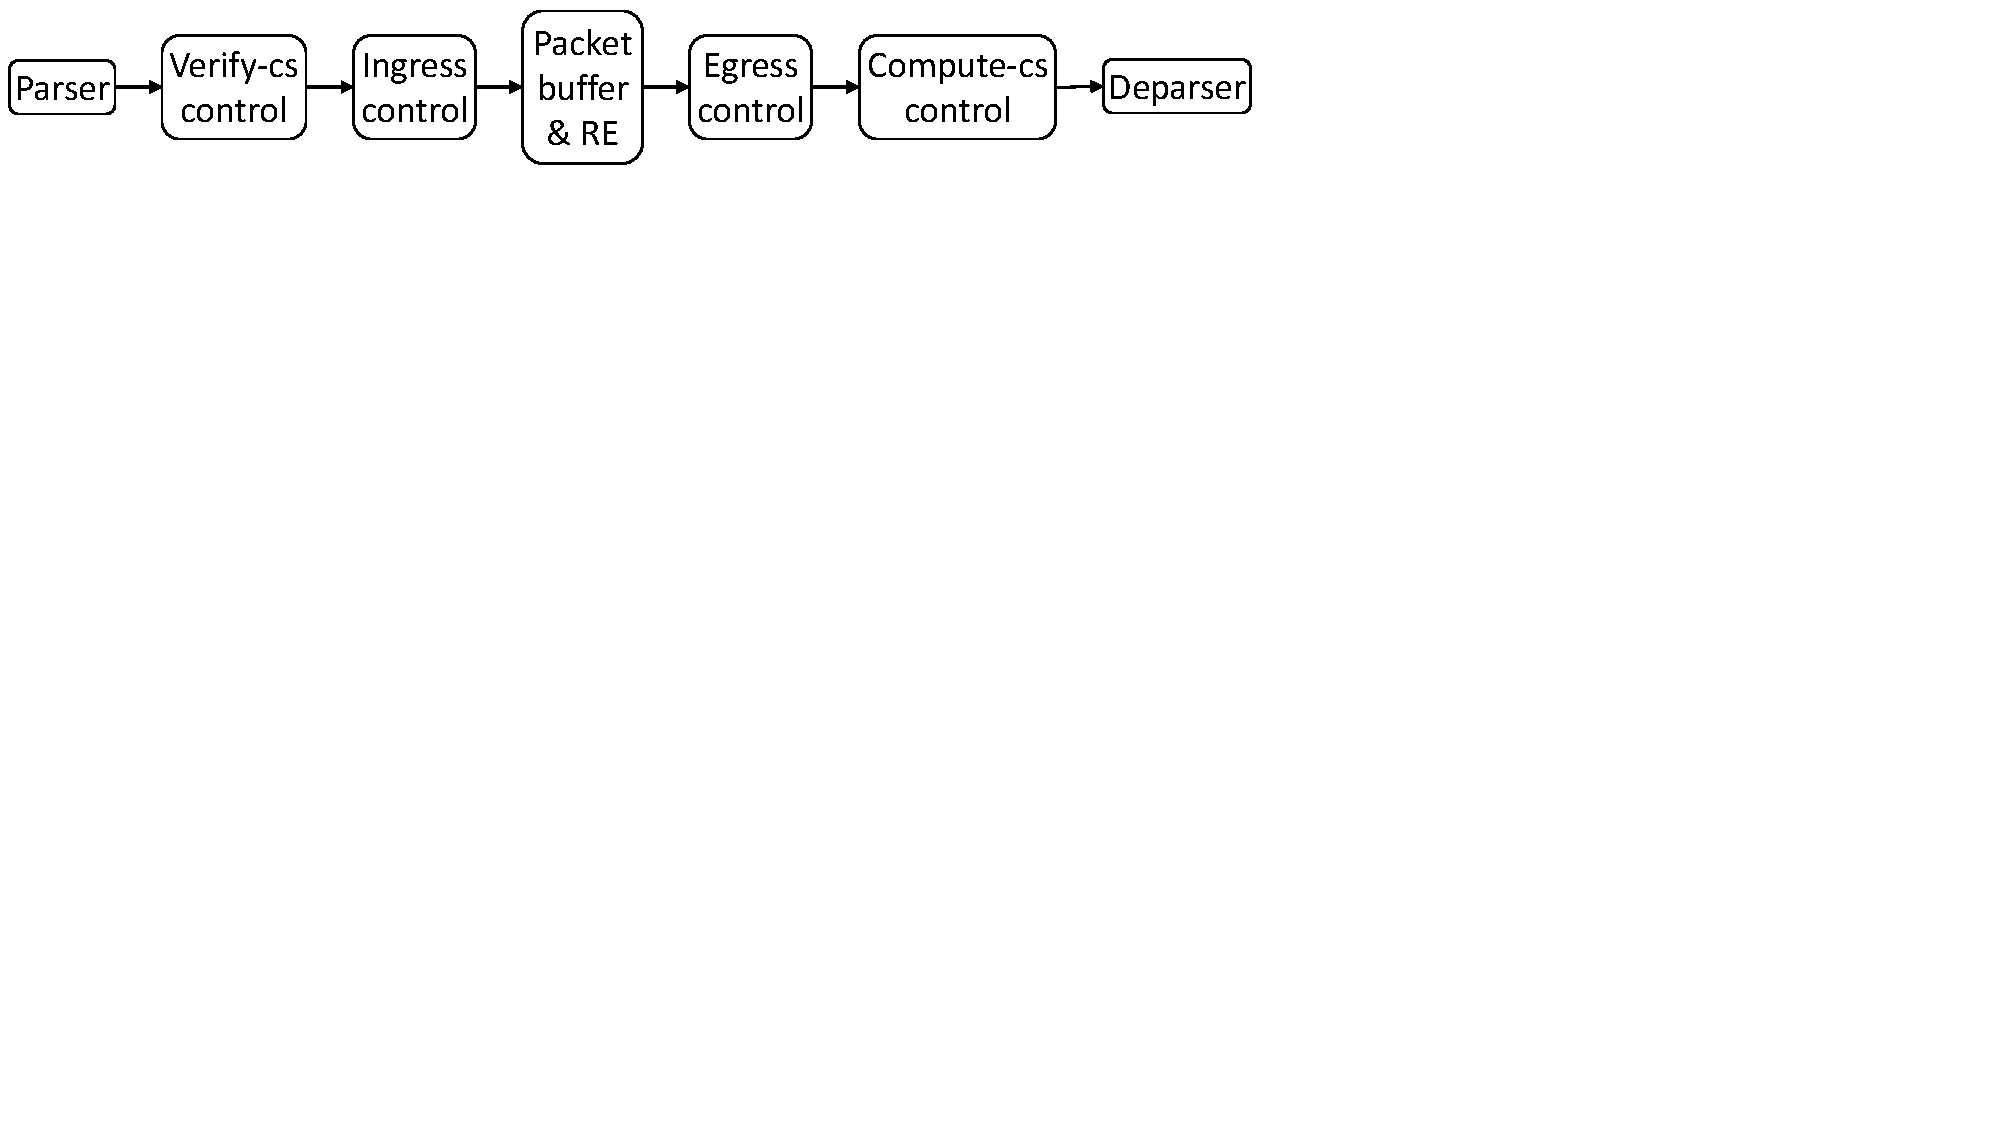
\includegraphics[trim=3 460 357 0, clip,scale=0.35]{v1model-pipeline.pdf}
%  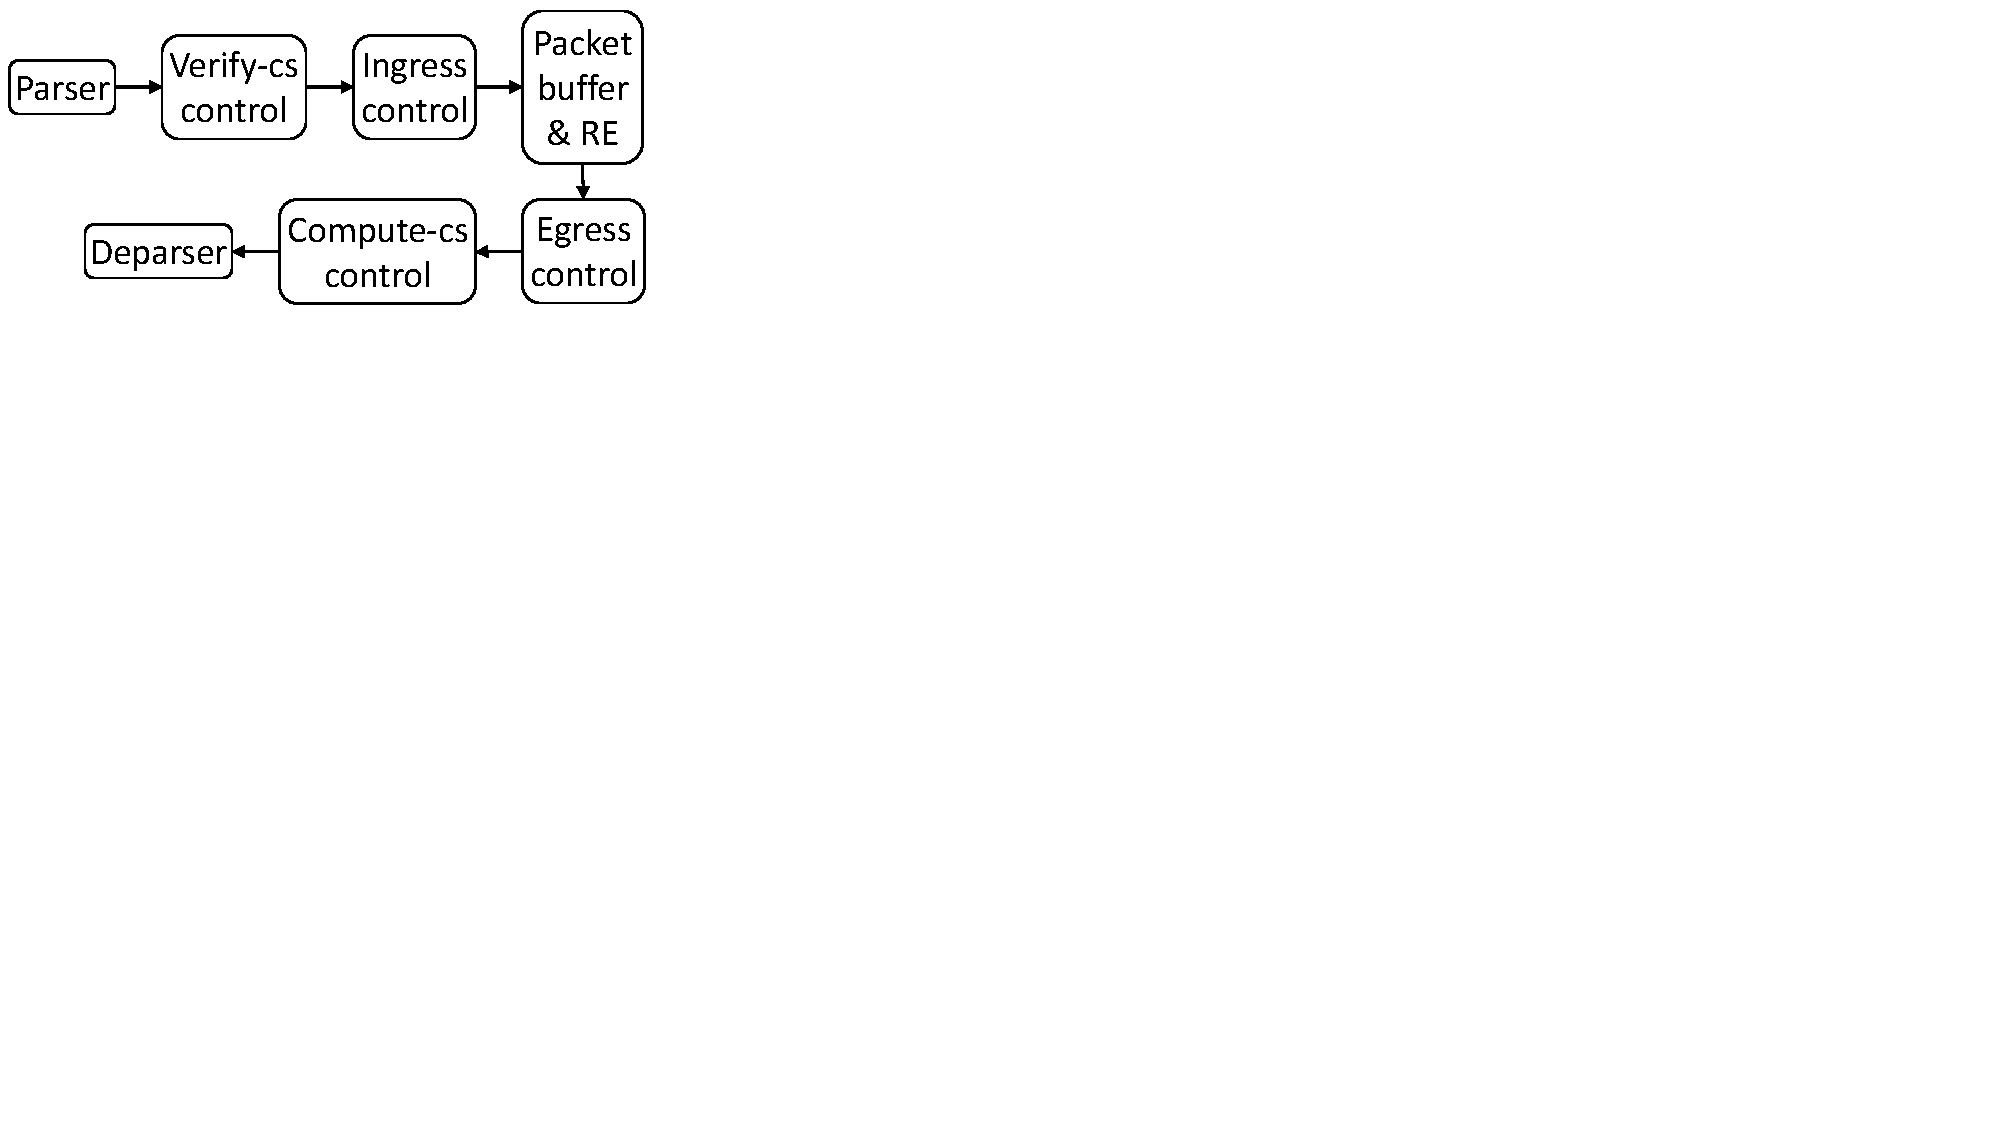
\includegraphics[trim=0 390 650 0, clip,scale=0.5]{v1model-pipeline-wrap.pdf}
%  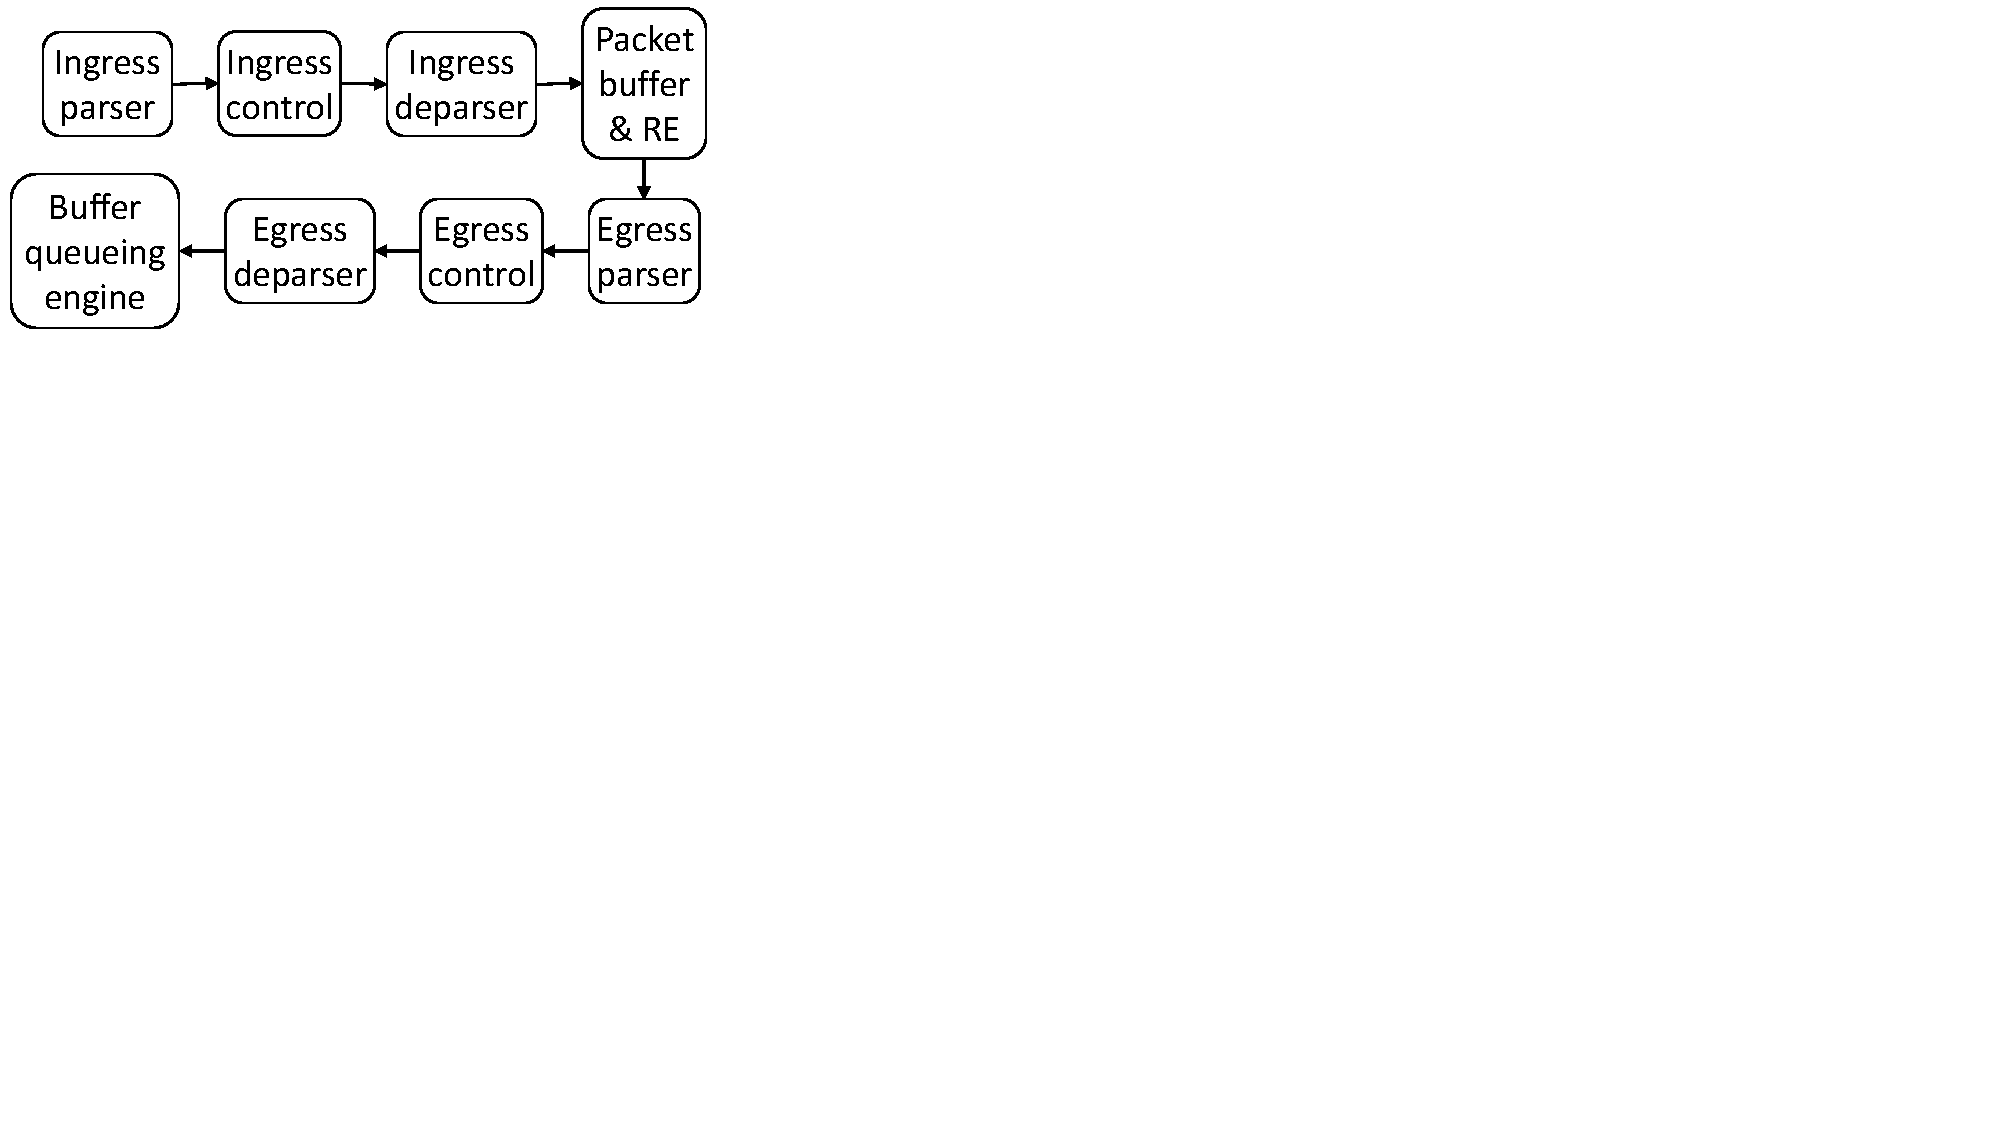
\includegraphics[trim=0 380 620 0, clip,scale=0.5]{psa-pipeline-wrap.pdf}
%  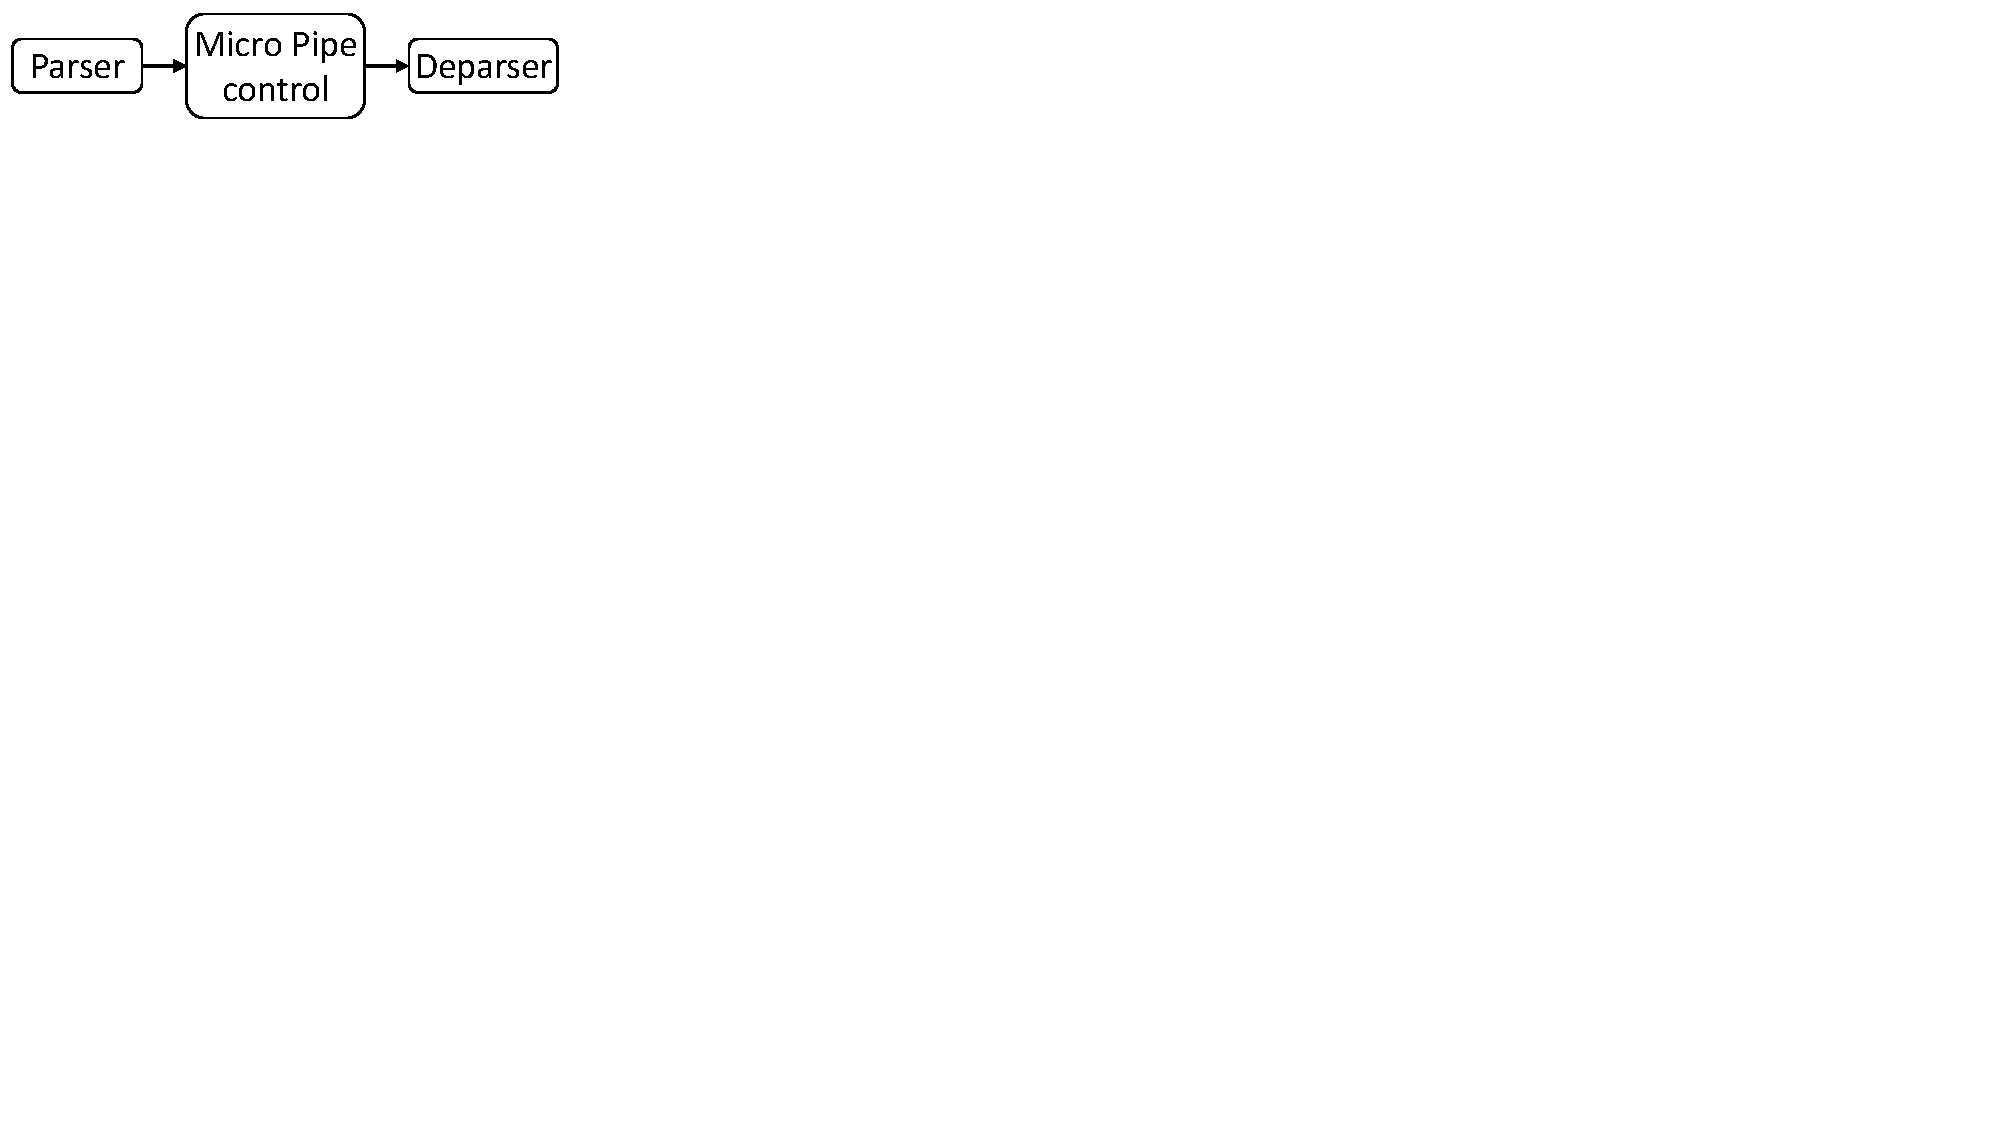
\includegraphics[trim=0 482 692 0, clip,scale=0.7]{msa-pipeline.pdf}
%  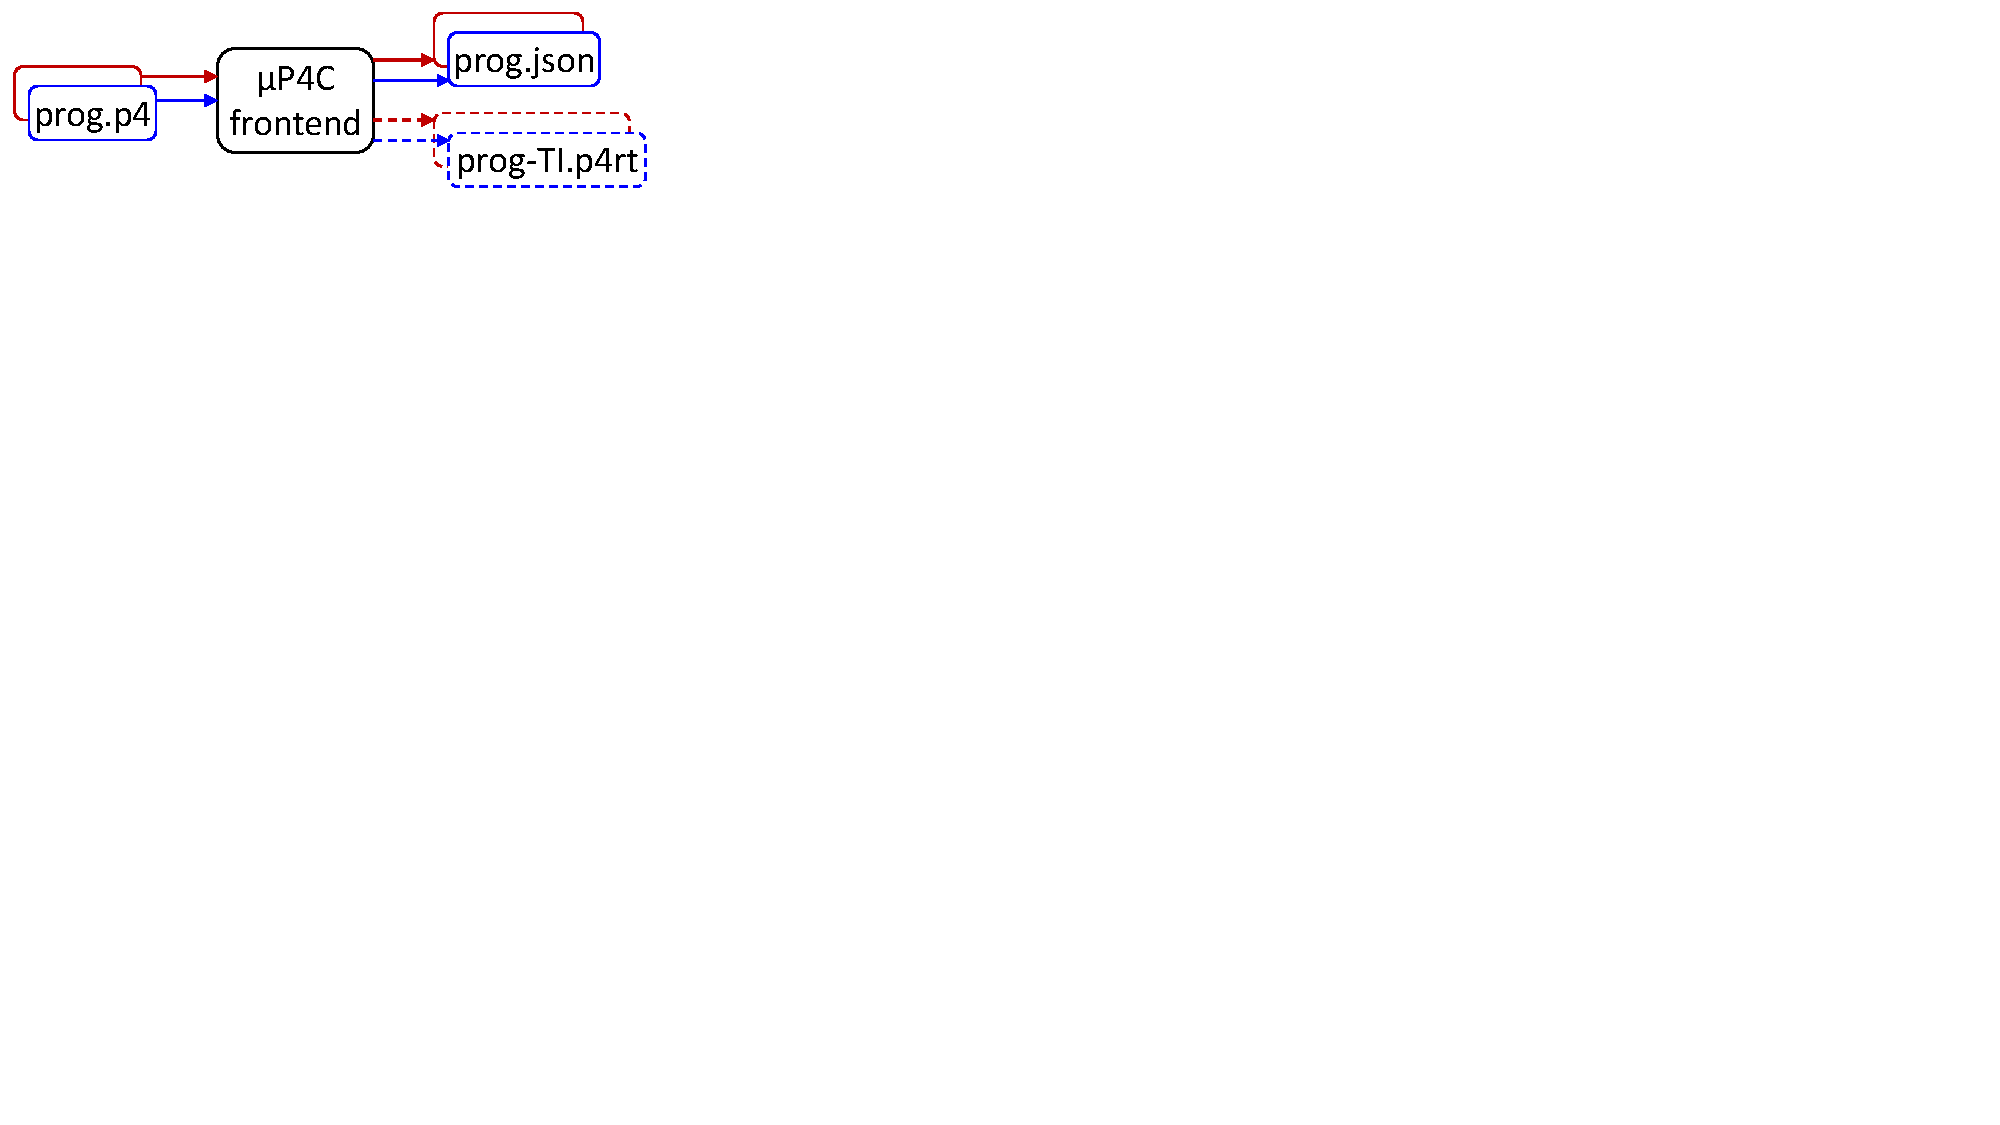
\includegraphics[trim=0 450 645 0, clip,scale=0.6]{mp4c-frontend.pdf}
%  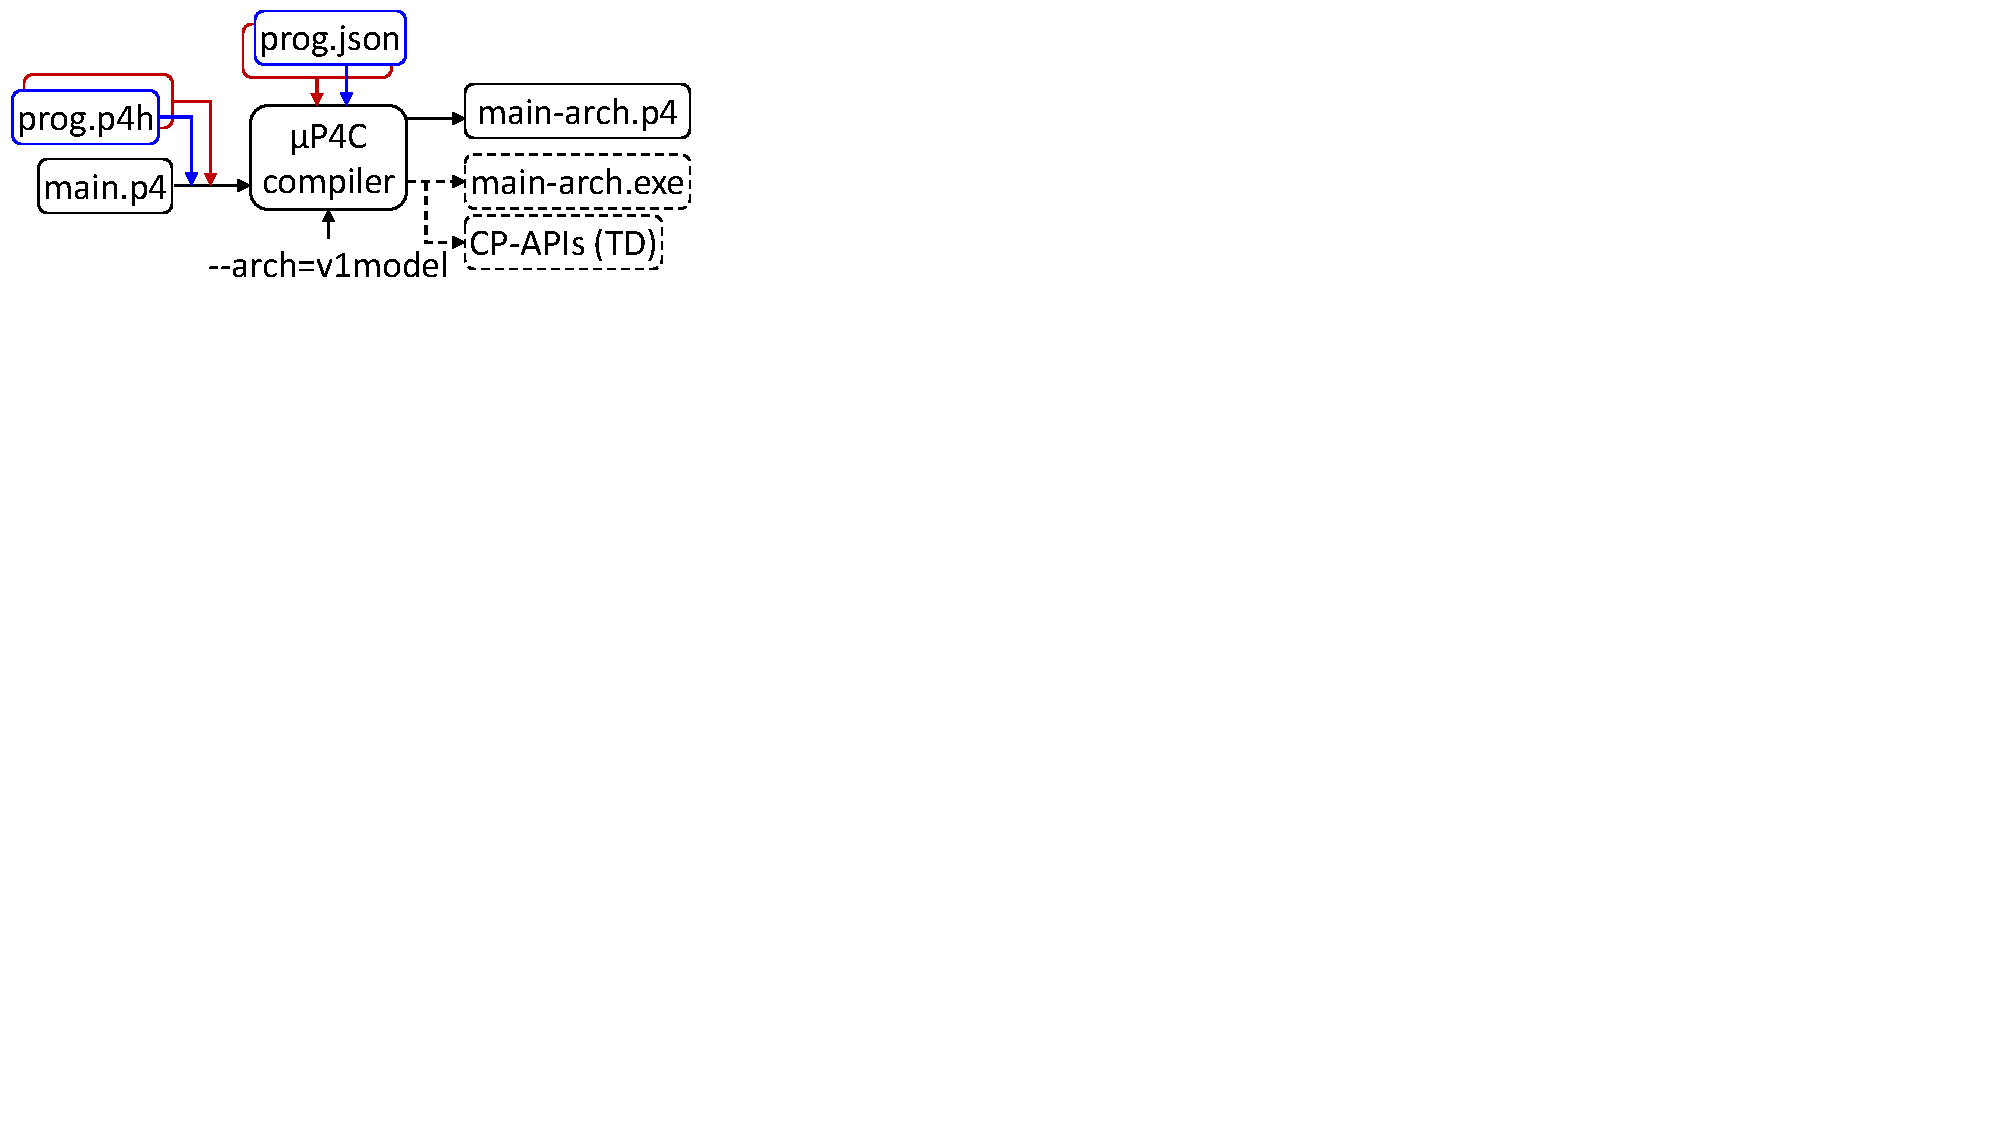
\includegraphics[trim=0 405 623 0, clip,scale=0.7]{mp4c-compiler}
%  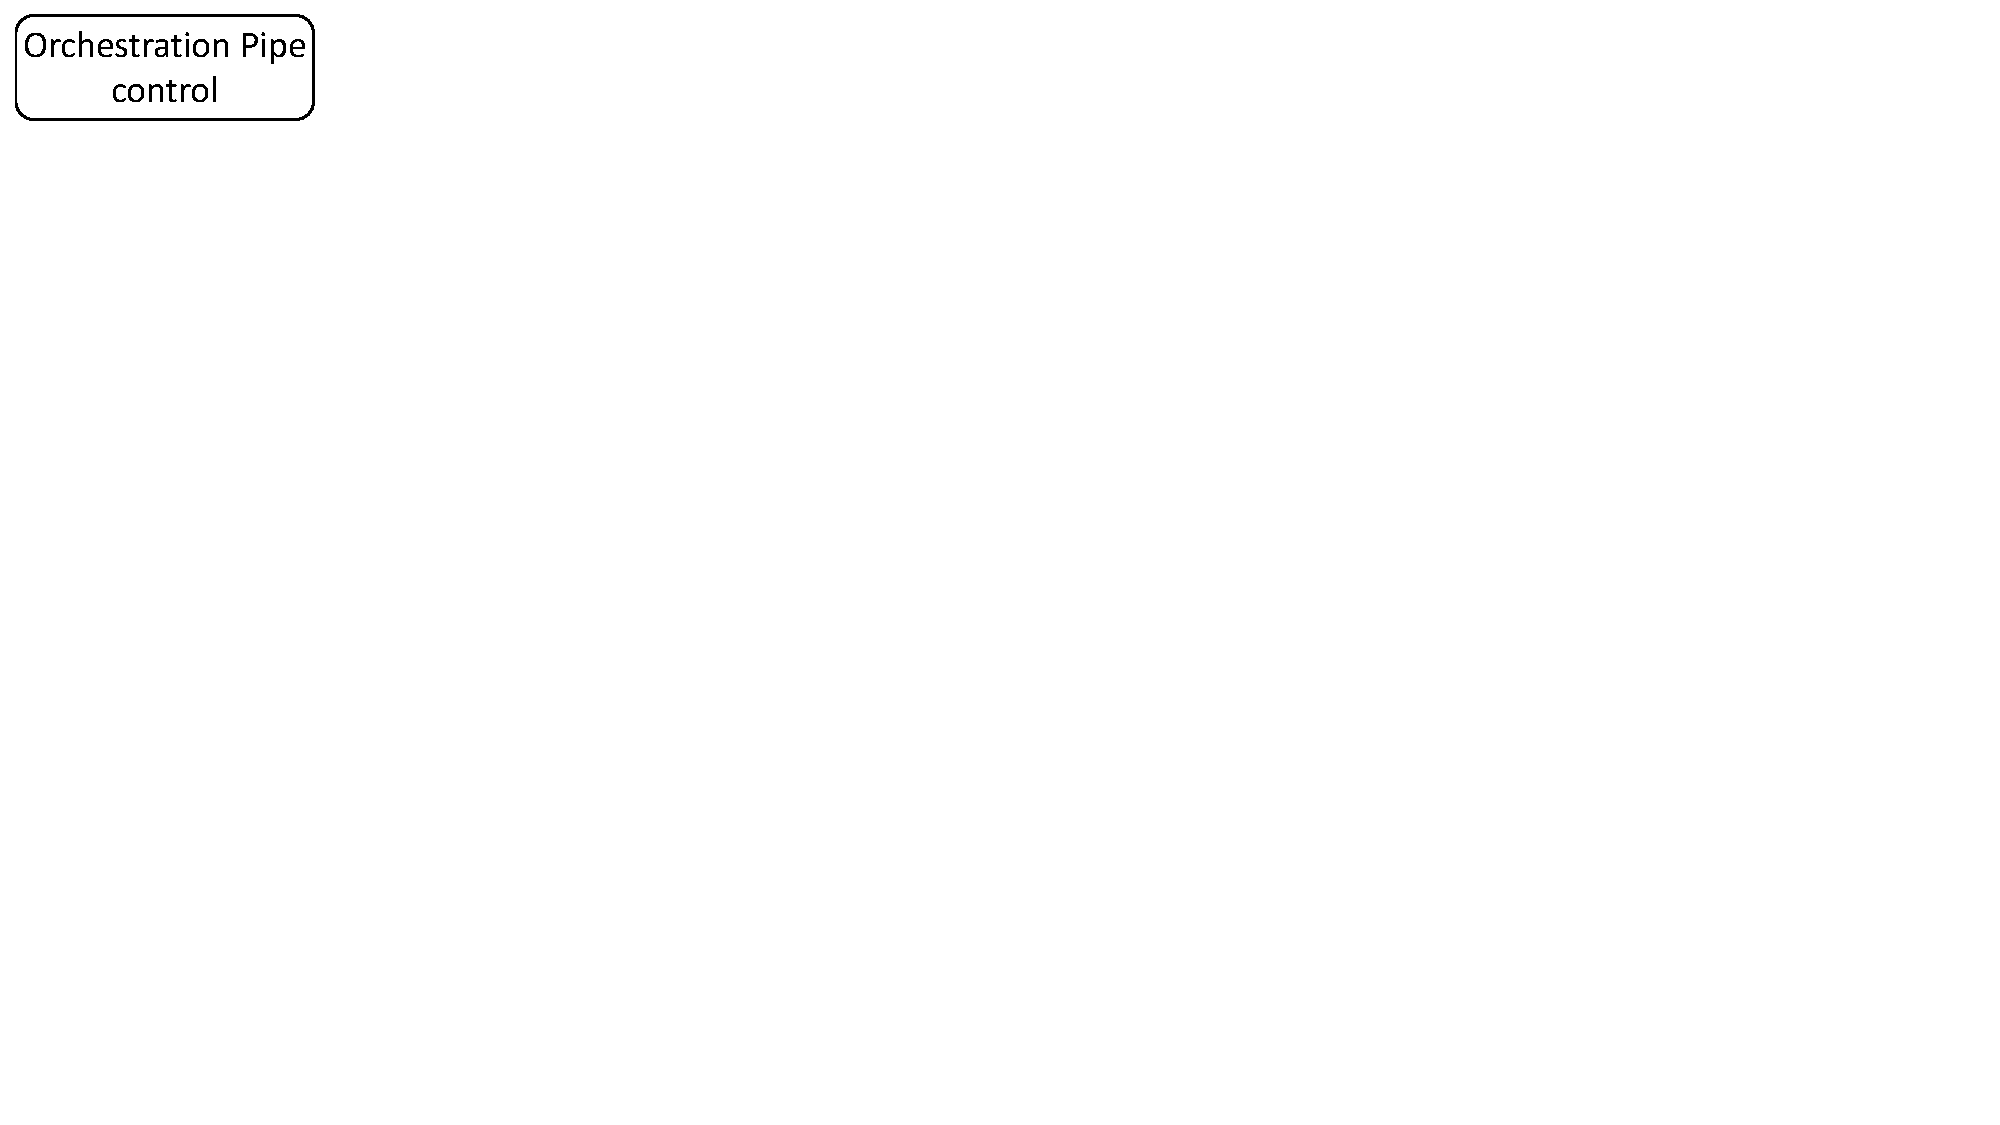
\includegraphics[trim=0 480 805 0,clip,scale=0.5]{micro-orchestration-pipeline}
% \end{figure}

\section{Overview Micro-P4 \;($\mu$P4)}
\label{section:overview-micro-p4}
% Re-configurable targets process packets using multiple type of processing blocks and P4 provides multiple sub-languages following heterogenous abstract machines to program the blocks.
% The presence of heterogeneous abstract-machines and device-specific constructs is the
% primary reason for lack of mechanisms for modularity and code reuse.
% Because, it is not possible to define interface to reuse code modules when caller and callee modules can have incompatible abstract machines.

$\mu$P4 is a logical device providing abstraction for packet-processing pipelines in data planes of real target devices.
$\mu$SA specifies data plane architecture of the logical device.
$\mu$P4C compiles $\mu$P4 programs to real target device's architecture-specific code.
% $\mu$SA simplifies abstract machine for P4 data plane programs by exposing minimal number of programmable blocks required to implement.
It declares logical externs that allows programmers to express packet-processing logic relying on fixed-function blocks in real targets.
The generic interfaces declared in $\mu$SA allow to reuse code of fine-grained packet-processing functions on any real target devices.
We associate runtime behavior with the interfaces.
$\mu$P4C allows programmer to define, instantiated and invoke them package types using \texttt{apply} method calls.
% Also, programmers can build new functions using the code.
Using the generic interfaces along with logical externs, programmers can express \emph{sequential}, \emph{parallel} and \emph{multicast} exection of packet-processing functions to build new programs.
$\mu$P4C enables composition of packet-processing functions using P4 language itself \hs{in related work}\emph{without relying on different configuration languages like Hyper4 and P4Visor}.
It translates simplified abstract machine and its logical externs into real target-specific heterogeneous packet-processing blocks, features and constraints.
In this section, we introduce packet-processing model of $\mu$P4, generic interfaces and operation concepts.

\subsection*{Packet Processing Model}
\label{subsection:packet-processing-using-mp4}
We model every packet-processing function as a black-box micro-switch that processes packet byte-stream, intrinsic metadata and arguments for user-defined parameters, as shown in Figure \ref{fig:mp4-packet-processing-model}.
The black-box model hides implementation details (headers types, user-defined metadata, programmable blocks etc.,) of micro-switch programs.
We augment micro-switch programs with input and output buffer queues.
Each element in the queue contains a packet byte-stream, intrinsic metadata associated with it and arguments.
In this model, the micro-switch program fetches an element from the input buffer to process at every execution step.
As a result of the processing, the program may generate one or more elements.
We enqueue them in output buffer queue.
\begin{figure}
    \centering
    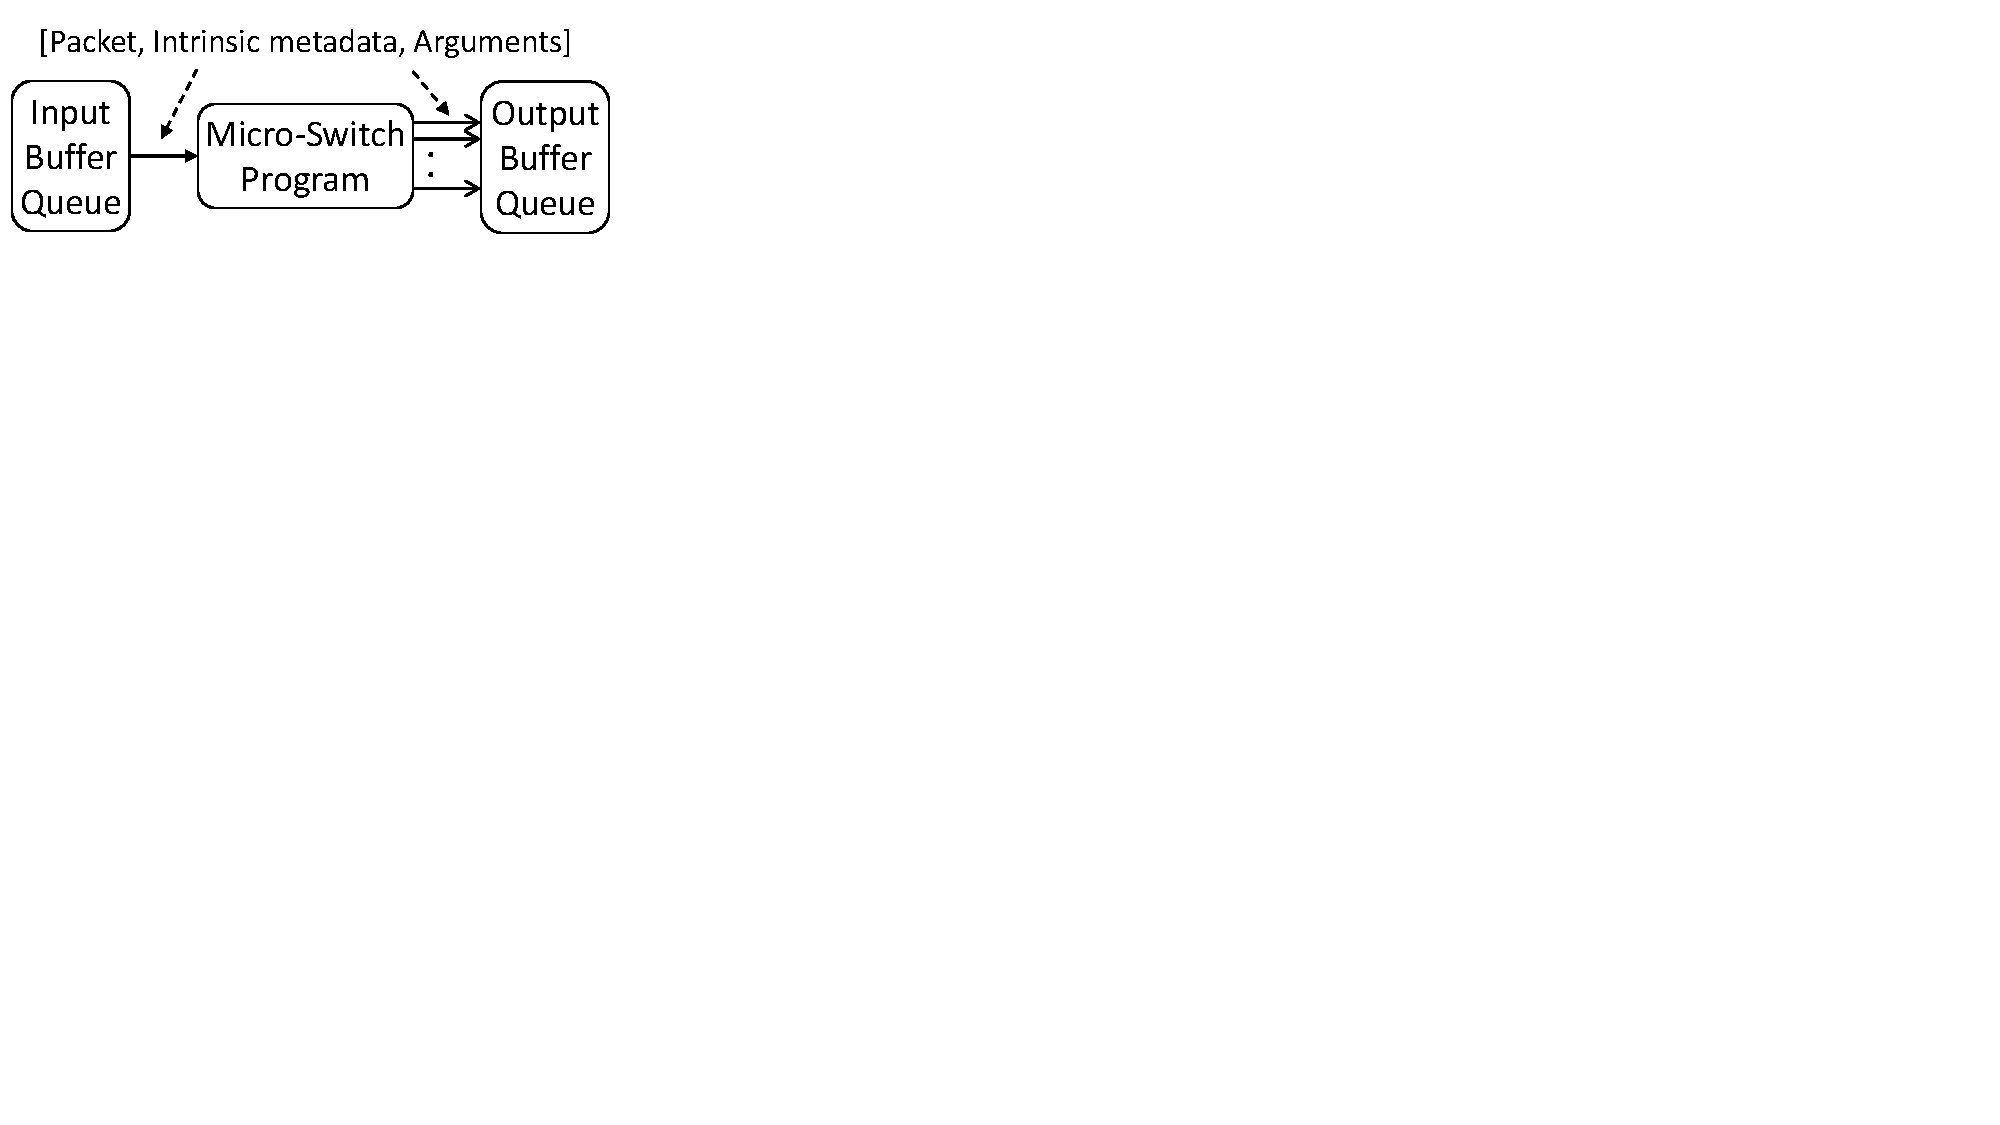
\includegraphics[trim=0 420 667 0, clip, scale=0.5]{microp4-program-model}
    \caption{$\mu$P4 Packet Processing model}
    \label{fig:mp4-packet-processing-model}
\end{figure}

To realise this model, $\mu$SA defines multiple packet-pro\-cessing pipelines and each pipeline is associated with one or more generic interface types.
Each generic interface declares a set of programmable blocks to implement based on the associated pipeline model.
The interfaces allow programmers to specify user-defined types for the runtime parameters.
Programmers can implement the interfaces to define new \texttt{package} types.
This user-defined package types can be instantiated and invoked in control blocks of $\mu$SA pipelines.
Programmers have to declare package types, defined in other code libraries, with their concrete runtime interfaces to use in the current program.
Next, we describe compilation procedure that facilitates reuse of user-defined package types.


\subsection*{Compiling $\mu$P4 Programs}
$\mu$P4C provides well-known mechanism, compile and link, to generate executable code.
If a program does not contain main instance, $\mu$P4C generates a library by compiling it to an Intermediate Representation (IR) in json format (Figure \ref{subfig:compiling-modules}).
It also generates architecture-independent control-plane APIs, P4Runtime \cite{p4runtime} files.
% $\mu$P4C's front-end generates P4Runtime files containing only APIs for match-action tables in the program.
% The front-end of $\mu$P4C resolves used-package types with their declarations or definitions.
\begin{figure}
    \centering
    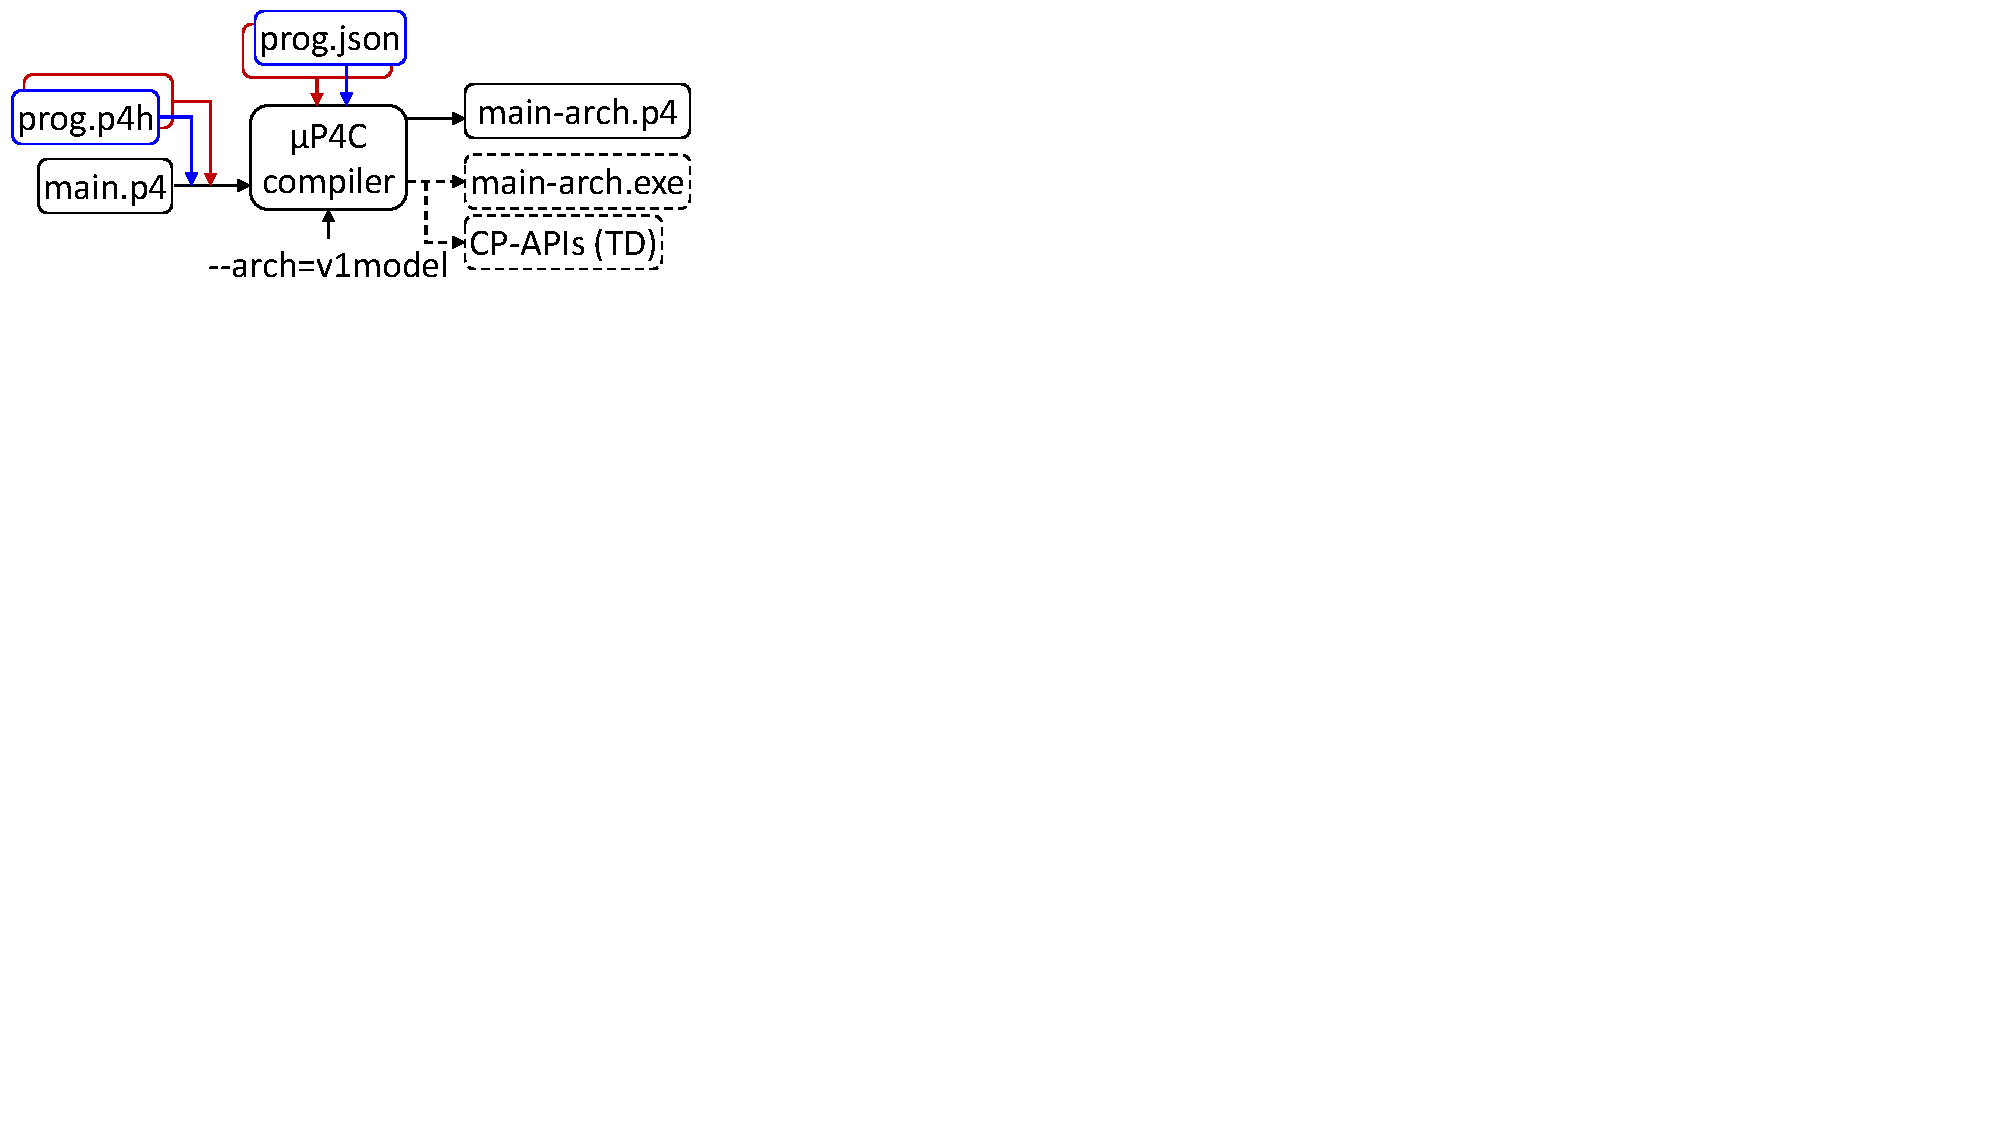
\includegraphics[trim=4 350 633 4, clip,scale=0.45]{mp4c-compiler}
    \caption{Compiling $\mu$SA programs}
\label{fig:compiling-msa-programs}
\end{figure}
Programmers can include files containing definitions of types (e.g., struct types of in and out parameters) used in runtime interfaces of packages in libraries.
$\mu$P4C compiler generates either source P4 code for the specified architecture or executable with architecture-specific CP APIs.

\hs{next we describe msa and mp4c...}



\section{Micro-Switch Architecture}
\label{section:micros-awitch-architecture}
The design goals behind $\mu$SA are $(1)$ provide logical abstraction for data plane pipelines without compromising expressiveness and packet-processing features, $(2)$ declare generic interfaces to allow easy code reuse and enable modularity.
First, we describe logical pipelines of $\mu$P4. Then, we introduce $\mu$SA's externs and generic interfaces along with example usages.

% This design choice reduces heterogeneity in abstract model of data plane programs.
% For each pipeline type, it exposes an interface type comprising a set of programmable blocks.
% Programmers can define a P4 \emph{package} type by implementing all the programmable blocks of a interface type.
% In the same source file, programmers can provide multiple implementations of the same interface type to define multiple package types.
% $\mu$SA defines various architecture specific structures and externs that allow programmers to express sequential and parallel composition of fine-grained packet processing functions.

% It defines standard intrinsic metadata as \emph{msa\_sm\_t} as a struct type.
% The fields of this struct provide basic information populated by the target e.g., \emph{packet\_length}.

% Some fields are not mutable, however $\mu$SA allows to declare instances of the struct and perform assignment operation between two instances to create copies.
% Sections \ref{subsection:pipelines} and \ref{subsection:logical-externs} describe pipelines and logical externs, respectively.



\subsection{Pipelines}
\label{subsection:pipelines}
$\mu$SA has two types logical pipeline, Micro and Orchestration, shown in Figure \ref{fig:msa-pipelines}
$\mu$SA provides a set of logical externs which can be instantiated and used within control blocks of the $\mu$SA pipelines.
% Micro pipeline comprises of Parser, Micro-Pipe control and Deparser programmable blocks.
% Every incoming packet is parsed and validated by the parser, if parser terminates in \texttt{accept} state, then execution-control is transferred to micro-pipe control block.
% Depending on use of logical externs in implementation, packet may not complete the processing of the control block.
If the execution-control reaches till the end of the control block, packet is processed by the deparser block.
\begin{figure}
    \centering
    \begin{subfigure}{0.59\linewidth}
        \centering
        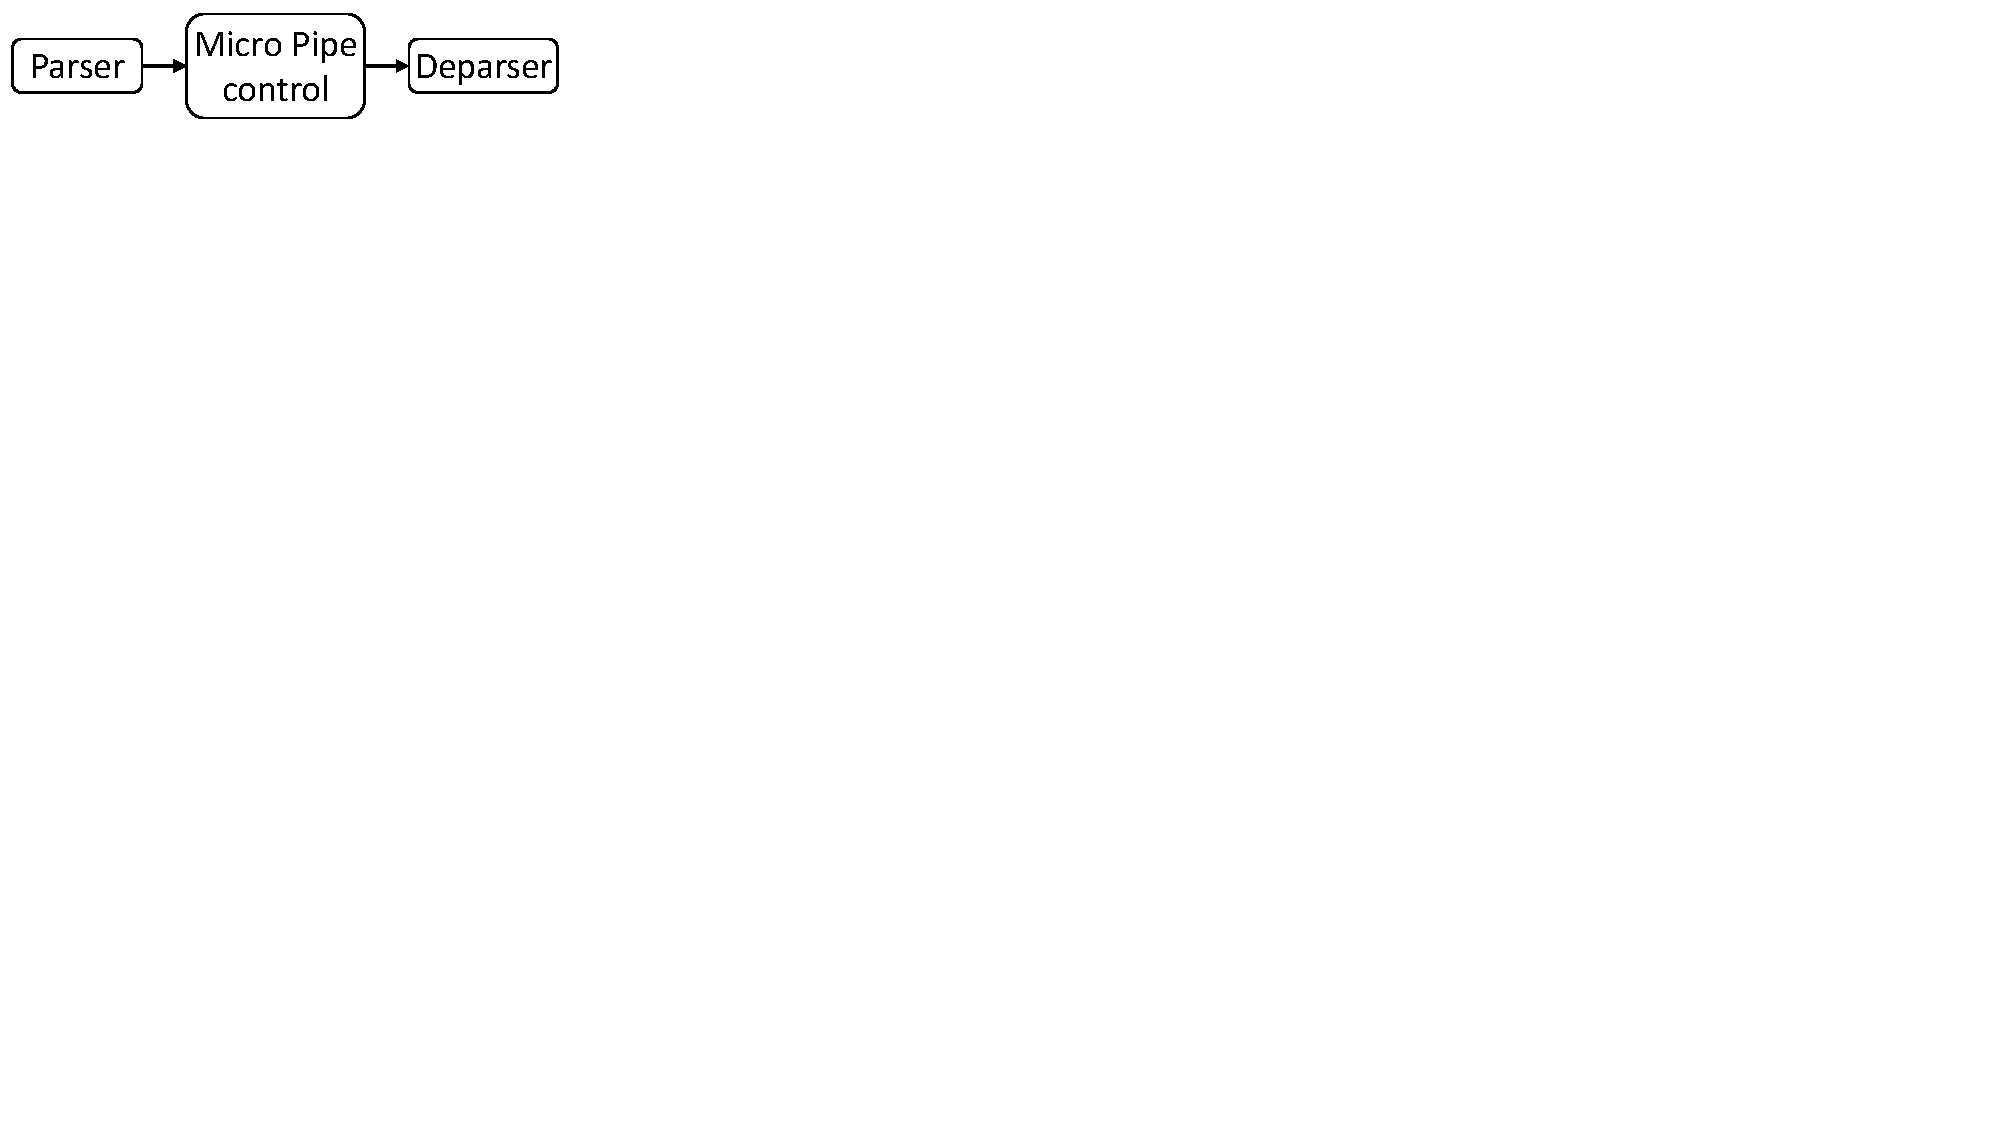
\includegraphics[trim=0 482 692 0, clip,scale=0.45]{msa-pipeline}
        \caption{Micro}
%         \label{subfig:micro}
    \end{subfigure}\vline
    \begin{subfigure}{0.41\linewidth}
        \centering
        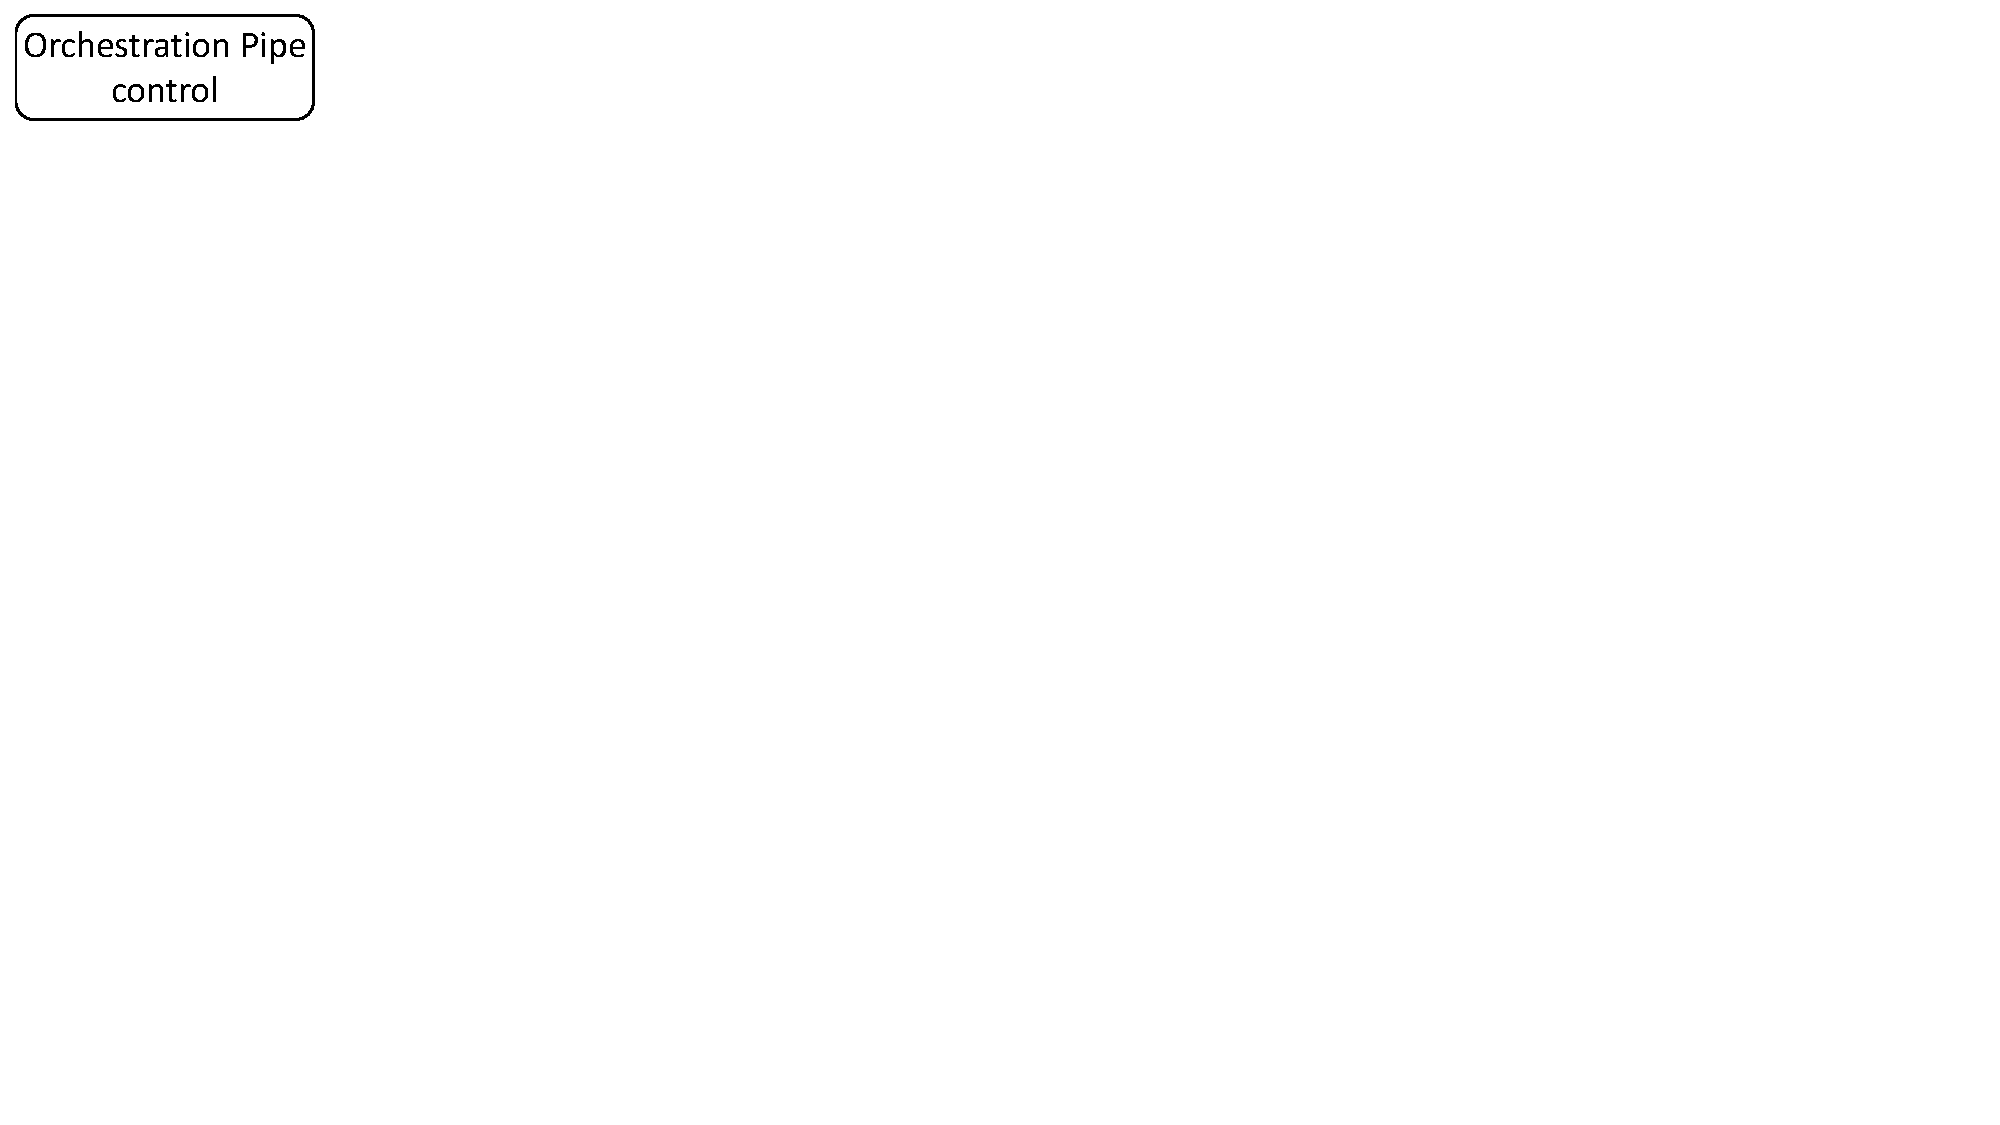
\includegraphics[trim=0 480 805 0,clip,scale=0.45]{micro-orchestration-pipeline}
        \caption{Orchestration}
%         \label{subfig:orchestration}
    \end{subfigure}
\caption{$\mu$SA Pipelines}
\label{fig:msa-pipelines}
\end{figure}
% \vspace{-3pt}
Orchestration pipeline only has a control block, orchestration pipe.
Programmers can implement imperative control flow using intrinsic metadata of $\mu$SA and runtime parameters to the package types.

Figure \ref{fig:interfaces} shows signature of type-parameterised interfaces declared in $\mu$SA.
Unicast (U) and Multicast (M) interface can be implemented using Micro pipeline.
General (G) interface allows to implement Orchestration pipeline.
In Figure \ref{fig:interfaces}, \texttt{pkt\_in} and \texttt{pkt\_out} represent packet, \texttt{sm\_t} and \texttt{es\_t} represent intrinsic metadata.
\texttt{in\_buf} and \texttt{out\_buf} externs represent input and output buffer of $\mu$P4 packet-processing model (Figure \ref{fig:mp4-packet-processing-model})
% \vspace{-7pt}
\begin{figure}
\begin{lstlisting}[frame=none]
U<I, O, IO>(pkt_in, pkt_out, inout sm_t, es_t, in I, out O, inout IO); 
M<O>(pkt_in, in sm_t, es_t, out_buf<O>);
G<I, O>(in_buf<I>, out_buf<O>);
\end{lstlisting}
\caption{Runtime Interfaces}
\label{fig:interfaces}
\end{figure}
% \vspace{-10pt}

\subsection{Logical Externs and Examples}
% We declare a set of externs to enable packet-processing model described in \ref{section:overview-micro-p4}.
% Every micro-switch program process on packet, intrinsic metadata and argument.
% Program needs to pass instance of externs representing packet to invoke micro-switch program.
% A
% $\mu$SA declares pkt\_in and pkt\_out externs containing instances of their counterpart in core library.
% 
% 
% $\mu$SA specific packet externs \emph{msa\_packet\_in} and \emph{msa\_packet\_out} contain an instance of \emph{packet\_in} and \emph{packet\_out}, respectively.
% We introduce a function, \emph{get\-\_packet\-\_in}, in \emph{msa\-\_packet\-\_out}.

% \begin{lstlisting}[frame=none]
% void get_pkt_in(pkt_in pi);
% \end{lstlisting}
% Similarly, we introduce copy\_from function in \emph{msa\_packet\_in} that replicates the state of passed argument (\emph{msa\_pin}) to the calling instance.
% \begin{lstlisting}[frame=none]
% void copy_from(pkt_in pi);
% \end{lstlisting}

\subsubsection{Egress Specifications}
Many packet-processing devices allow to measure every packet's queuing latency through the device.
These timestamps required to compute queuing latency can be measured only after the packet's egress port is finalized.
The timestamps can be accessed only after the egress port is finalized.
$\mu$SA captures such constraints as using stateful extern objects capturing data-dependency.
% To support such special features, the architectures of real target devices expose intrinsic metadata  that depends on operations on other intrinsic metadata.
\begin{figure}
\begin{minipage}[c]{0.27\linewidth}
\begin{lstlisting}[frame=none]
enum meta_t {
  INGRESS_TS,
  EGRESS_TS
}
\end{lstlisting}
\end{minipage}\vline\hspace{3pt} 
\begin{minipage}[c]{0.68\linewidth}
\begin{lstlisting}[frame=none]
extern es_t {
  void set_egress_port(in bit<8>);
  bit<8> get_egress_port();
  bit<32> get_value(in meta_t ft);
  void copy_from(es_t es);
}
\end{lstlisting}
\end{minipage}
\caption{Extern to Capture Data-Dependency(Egress\_Spec)}
\label{fig:msa-egress-spec-extern}
\end{figure}
$\mu$SA declares \texttt{es\_t} as an extern object (Figure \ref{fig:msa-egress-spec-extern}).
It declares methods to manipulate and access interdependent device-specific information.
$\mu$P4C uses their occurrences to transform the code to multi-control pipelines of real target architectures.

% $\mu$P4C allows repeated usage of the extern's functions in the single control block of $\mu$SA pipelines.
% If \emph{get\_value} occurs before \emph{set\_egress\_port} on any possible execution-control path, $\mu$P4C raises a compile-time error.


\subsubsection{Packet Externs}
We use an example of sequential exection to introduce additional methods declared in pkt\_in and packet\_out compared to packet externs of P4 core library \cite{core.p4}.
In sequential processing, packet processed by one program is passed to another.
Figure \ref{fig:sequential-execution} illustrates reuse of the code shown in Figure \ref{fig:l3.p4.l2.p4} to build a routing function, called \texttt{l2l3}.
The unicast interface defined in Figure \ref{fig:interfaces} is used for both programs.
Notice the use of \texttt{get\_pkt\_in} method that provides conversion between pkt\_in and pkt\_out externs to express sequential packet-processing.
% $\mu$P4 allows programmers to invoke micro-switch programs using their interfaces in body of control blocks other micro-switch program.
% \vspace{-10pt}
\begin{figure}
\begin{lstlisting}[frame=none]
// declarations for l3 and l2
l3(pkt_in, pkt_out, sm_t, es_t, out bit<16>);
l2(pkt_in, pkt_out, sm_t, es_t, in bit<16>);
control l2l3(pkt_in pin, pkt_out po, 
             sm_t s, es_t e) {
  bit<16> next_hop; pkt_in pin_l2;
  apply {
    l3.apply(pi, po, s, es, next_hop);
    // sets `pin_l2' with `po's bytes, resets `po'
    po.get_pkt_in(pin_l2); // extern method call
    l2.apply(pin_l2, po, s, es, next_hop);
  }
}
\end{lstlisting}
\caption{Sequential Execution}
\label{fig:sequential-execution}
\end{figure}
% \vspace{-10pt}

\subsubsection{Packet Buffer}
We take an example of parallel processing to introduce externs objects representing packet buffers.
$\mu$P4 allows programmer to create copies of packets, intrinsic metadata and arguments and pass each copy to a different program.
Figure \ref{fig:parallel-execution} shows a program, called \texttt{rm}, executing \texttt{l2l3} (Figure \ref{fig:sequential-execution}) and \texttt{mirror} (traffic sampler) in parallel.
% Programmers can use assignment statements to create copies of standard intrinsic metadata (msa\_sm\_t) and use \emph{copy\_from} functions in \emph{msa\_packet\_in} and \emph{egress\_spec} to create copies of the packet and intrinsic metadata.
$\mu$SA declares buffer externs \texttt{in\_buf} and \texttt{out\_buf} with \texttt{dequeue} and \texttt{enqueue} methods, respectively.


The buffers can only be instantiated in the control block of orchestration pipeline.
Its functions can be used only in apply body of the control block.
% The output of the multiple programs generated by processing the same packet can be enqueued in the logical buffer.
Multiple dequeue calls would result in weighted traffic split.
% /*
% extern msa_packet_buffer<ET> {
%   msa_packet_buffer();
%   void enqueue(pkt_out po, in sm_t sm, es_t es, in ET data);
%   void dequeue(pkt_in pin, out sm_t sm, es_t es, out ET data); 
% }
% */
% \begin{figure}[!h]
% \begin{lstlisting}[frame=none]
% extern out_buf<T> {
%   void enqueue(pkt_out po, in sm_t sm, es_t es,
%                in T data); 
% }
% extern in_buf<T> {
%   void join(out_buf<T> ob);
%   void dequeue(pkt_in pi, out sm_t sm, es_t es, 
%                out T data); 
% }
% \end{lstlisting}
% \caption{Packet Buffer Extern}
% \label{fig:msa-packet-buffer-extern}
% \end{figure}
% In parallel execution of multiple micro-switch programs, each program processes its own copy of a packet.
% Programmers can create copies of a packet using logical constructs defined in $\mu$SA.
.
\begin{figure}
\begin{lstlisting}[frame=none]
extern out_buf<O> {
  void enqueue(pkt_out, in sm_t, es_t, in O); 
}
extern in_buf<I> {
  void dequeue(pkt_in, out sm_t, es_t, out I); 
}

// interface for traffic mirror function
mirror (pkt_in, pkt_out, sm_t);
l2l3 (pkt_in, pkt_out, sm_t); struct e_t {};
control rm(in_buf<e_t> ib, out_buf<e_t> ob) {
  pkt_in pin, pin_m; es_t es_m;
  pkt_out po_m; sm_t sm, sm_m;
  apply {
    ib.dequeue(pin, sm, es);
    // copies for parallel execution
    pin_m.copy_from(pin); sm_m = sm; 
    es_m.copy_from(es)
    mirror.apply(pin_m, po_m, sm_m, es_m);
    l2l3.apply(pin, po, sm, es);
    // synchronize and put in out_buf arg
    ob.enqueue(po, sm, es);
    ob.enqueue(po_m, sm_m, es_m);
  }
}
\end{lstlisting}
\caption{Parallel Execution}
\label{fig:parallel-execution}
\end{figure}

% \subsubsection{Multicast Execution}
% \label{subsubsection:multicast-execution}
% Multicast execution differs from parallel execution in two fundamental aspects.
% $(1)$ Multicast execution allows to program packet replication at runtime.
% $(2)$ Each copy of the replicated packet executes the same code.
% % $\mu$SA defines a logical multicast engine, \texttt{mc\_engine\_t}, as an extern.
% Figure \ref{fig:multicast-execution} shows an example of expressing multicast replication using logical externs defined in $\mu$SA.
% \begin{figure}[ht]
% \begin{lstlisting}[frame=none]
% struct out_t { bit<16> data;}
% control mc(pkt_in pi, sm_t sm, es_t es, 
%         hs_t h, ia_t ia, mc_buf<hs_t, out_t> hb) {
%   mc_engine_t mce;  pkt_inst_id_t id; 
%   out_t  oa;
%   table t{
%     key = {} actions = { mce.set_mc_group; drop; }
%   }
%   table mac{
%     key = { es.get_port(); } 
%     actions = { mac_update; }
%   }
%   apply {
%     id = mce.apply(es); // equivalent to fork in C
%     mac.apply();
%     hb.enqueue(h, sm, es, oa);
%   }
% }
% control dep(pkt_out<o_a> ob, 
%             mc_buf<hs_t, out_arg_t> hb) {
%   hs_t hdrs; out_arg_t oa; pkt_out po;
%   hb.dequeue(hdrs, sm, es, oa);
%   // deparser code 
%   ob.enqueue(po, sm, es, oa);
% }
% \end{lstlisting}
% \caption{Multicast Execution}
% \label{fig:multicast-execution}
% \end{figure}


\subsubsection{Multicast Extern}
$\mu$SA's multicast extern (Figure \ref{fig:msa-multicast-extern}) can be instantiated in the control blocks of its pipelines.
The \emph{set\_multicast\_group} can be used to assign replication group to the packet. 
The \emph{apply} function is allowed to use only in \emph{apply} body control blocks. 
It is analogous to \emph{fork} system call in C except that processing of original packet terminates at the apply call.
It returns instance id of the replica and populates the es\_t instance with the port id set by the control plane.
$\mu$P4C translates this extern to multicast mechanism defined in architectures of real targets.
% We assume these architectures would have sufficient fields to program their replication engine, so that a combination of the fields can be used as packet instance id.
\begin{figure}
\begin{lstlisting}[frame=none]
extern msa_multicast_engine {
  msa_multicast_engine();
  void set_multicast_group(GroupId_t gid);
  PacketInstanceId_t apply(egress_spec es);
}
\end{lstlisting}
\caption{Multicast Extern}
\label{fig:msa-multicast-extern}
\end{figure}

\section{$\mu$P4C Compiler}
\label{section-mp4c-compiler}

\subsection{Parser Block Transformation}
\label{subsection:parser-block-transformation}
P4 parser blocks describe parse graphs as state machines.
Real target devices contain programmable parser module that can be programmed using parse graphs.
From the design of programmable parser~\cite{6665172}, we make following observations.
Programmable parsers are implemented using buffer, state machine logic, Ternary Content-Addressable Memories (TCAM) and Action RAM. 
TCAM matches values of current state, fields or variables to identify next state. 
Based on match, headers are copied from bit stream and current state is modified.
Programmable parsers essentially perform repeated match and action.
Also, we note that network packets are of finite length, hence they can be parsed in a finite number of ways.
Successful parsing of a packet is essentially finding a match for a finite number of bytes from finite set of values.
However, we need to extract all the bytes that might be required to perform match-actions from packets' bit streams.


We compute number of bytes required to extract in section~\ref{subsubsection:computing-size-of-byte-array}, followed by an approach to convert parser without loops and variable length headers, called \textit{simple parsers}, into a series of match-action tables.
Next, we explain loops unrolling and variable length headers removal techniques transforming every parser into a simple parser.
Finally, we discuss an optimization to reduce number of MATs to one.


\subsubsection{Computing Size of Byte Array}
\label{subsubsection:computing-size-of-byte-array}
% Every \emph{extract} method call statement in parser states advances bit index by number of bits equal to the size of the header type of the instance passed as the argument.
We perform symbolic execution of parser, control and deparser blocks to determine size of byte array buffer by evaluating call statements of \emph{extract} and \emph{emit} methods of core library externs \emph{packet\_in} and \emph{packet\_out}, respectively.
The symbolic execution also tracks validity of header instances by evaluating \emph{setValid} and \emph{setInvalid} method calls of P4 header types.
Symbolic execution of a parser block enumerates every possible path from the start to the accept state in the parse graph and computes total number of bytes extracted on every path.
We define length $l_{p}(x)$ of a path $x$ from the start to the accept state in the parse graph of program $p$'s parser as total number of bytes extracted.
And, the input buffer size for program $p$'s parser as $\mathcal{I}(p) = \max_{x}\left\{l_{p}(x)\right\}$. 


Programs may increase or decrease size of packets, therefore, considering only parser buffer size is not enough.
We perform symbolic execution of control and deparser blocks to determine maximum increase and decrease in packet size by the program.
We evaluate header instances' setValid and setInvalid method call statements on every path of the control flow graph.
We define worst case scenarios to estimate increase and decrese of size of packets on the same control path.
To estimate maximum decrement, we consider that a packet contains all the header instances that are set to valid or invalid on a control path.
Similarly for maximum increment, we consider that a packet does not contain any header instance that is set to valid or invalid on a control path. 
We denote increase and decrease in packet size on a path $x$ of control block of program $p$ using $i_{p}(x)$ and $d_{p}(x)$.
We define them as sum of sizes of all the header instances set valid and invalid on the path, respectively.
Header instances not emitted in any paths of deparser block by extracted by a parser state decrease packets size. 
For every path $x$, $d_{p}(x)$ is increamented by the size of such header instances. 
We define maximum decrease and increase in packet size by program $p$ as $\delta(p)$ and $\Delta(p)$, as shown in (\ref{decrease}) and (\ref{increase}).


\begin{align}
\delta(p)\; =& \;  \max_{x} \left\{ d_{p}(x) \right\} \label{decrease} \\
\Delta(p) \; =& \; \max_{x} \left\{ i_{p}(x) \right\} \label{increase}
\end{align}

To process packets by a sequence of $N$ programs, we define extract length, $\mathcal{E}l_{S}$ and buffer length $\mathcal{B}l_{S}$, as shown in (\ref{extract-length-seq}) and (\ref{buffer-length-seq}).
$\mathcal{E}l_{S}$ denotes the maximum number of bytes that may be extracted as cumulative effect of deparsers and parsers of all the program in a sequence.
$\mathcal{B}l_{S}$ denotes the maximum number of bytes that may be emitted as cumulative effect of the deparsers of all the programs in a sequence.
Similarly, we define extract length, $\mathcal{E}l_{P}$ and buffer length $\mathcal{B}l_{P}$, as shown in (\ref{extract-length-par}) and (\ref{buffer-length-par}), to process packets by $N$ programs in parallel.
\begin{align}
\mathcal{E}l_{S} \; =& \; \max_{i} \left\{ \left( \sum_{j=0}^{j<i} \delta(j) \right)+ \mathcal{I}(i) \right\},&\;\;\;i  \in [0,N] \label{extract-length-seq} \\
\mathcal{B}l_{S} \; =& \; \left( \sum_{i=0}^{N} \Delta(i) \right)+ \mathcal{E}l_{S} & \label{buffer-length-seq} \\
\mathcal{E}l_{P} \; =& \; \max_{i} \left\{ \mathcal{I}(i) \right\},&\;\;\;i  \in [0,N] \label{extract-length-par} \\
\mathcal{B}l_{P} \; =& \; \max_{i} \left\{ \mathcal{I}(i) + \Delta(i) \right\},&\;\;\;i  \in [0,N]  \label{buffer-length-par}
\end{align}


\subsubsection{Simple Parser to MATs}
\label{subsubsection:simple-parser-to-mats}
% We create action stage using parserStatements and match stage using ~\texttt{transitionStatement}.
Every path enumerated by symbolic execution of a parser consists of evaluated instances of the parser states.
A parser state can be a part of multiple paths, thereby having multiple instances.
% Every evaluated instance of a state provides a set of extracted (valid) header instances and their start bit indices corresponding to the state and the path.
P4 parser states consist of ~\emph{parser-Statements}  and \emph{transition\-Statement}.
The select expression in transition statement could be a header field, metadata or local variable declared in the parser.
The value of select expression of a state may depend on its ancestors' parser statements. <<as shown in diagram>>
Therefore, we perform Forward Substitution on select expressions in evaluated instances of states
% (https://dl.acm.org/citation.cfm?id=7904)
on each path and eliminate such data dependency.

We synthesise local binary variables, called \emph{visit},  for each parser state to track the state transition of the parser's FSM.
For every evaluated instance of a parser state, we synthesise an action comprising its parser\-Statements and replace extract method call statements to assignment statements.
The assignment statements copies bytes from the buffer array to header instances' fields according to their sizes.
Next, we add pop method call with the header size as the argument to remove the header from the byte array.
We insert setValid method call statement for the extracted header instances.
We add an assignment statement to set visit variable associated with the parser state.

\begin{figure*}[!h]
    \begin{subfigure}[b]{0.3\linewidth}
        \centering
        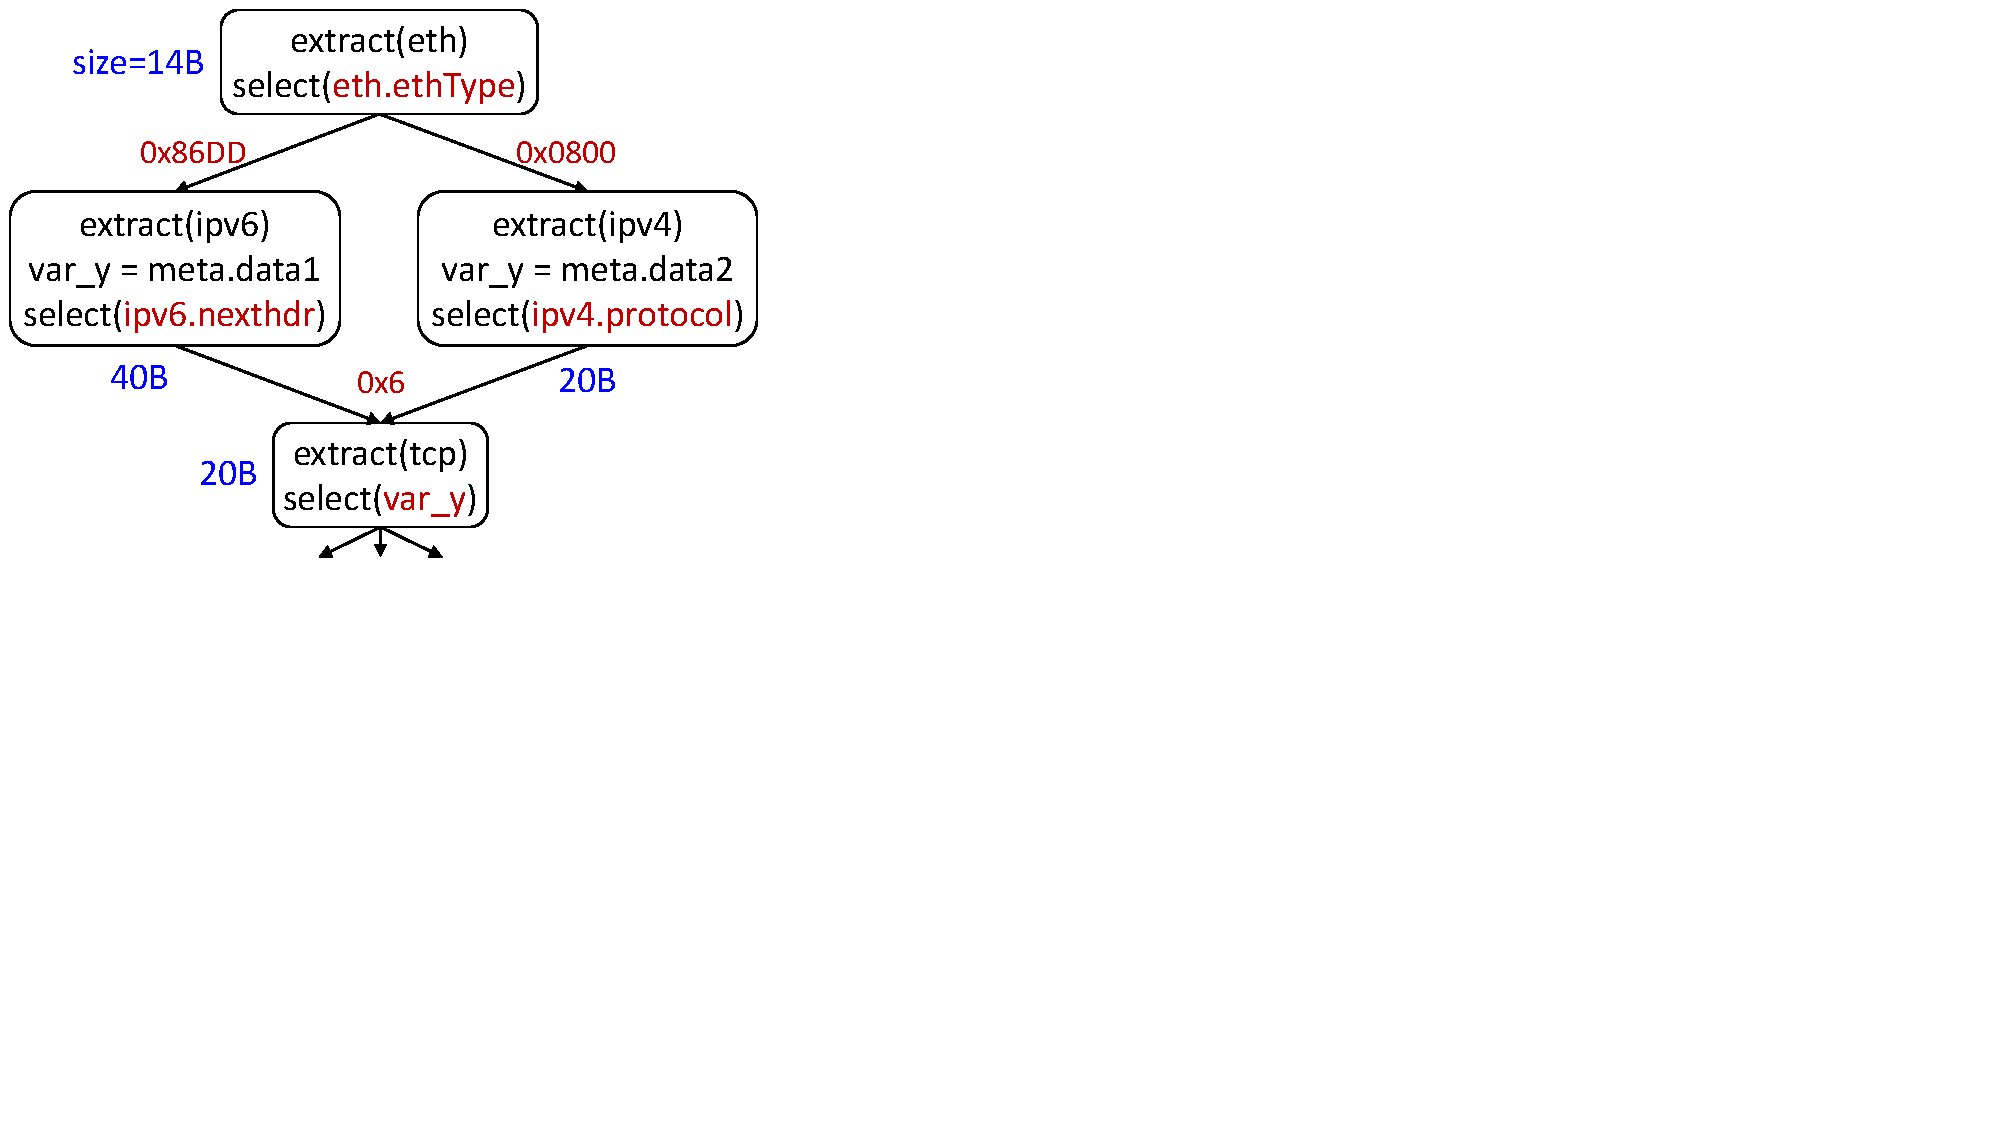
\includegraphics[trim=4 270 596 0, clip,scale=0.4]{parser-transformation-example}
        \caption{An example P4 Parser}
        \label{subfig:parser}
    \end{subfigure}
    \begin{subfigure}[b]{0.3\linewidth}
        \centering
        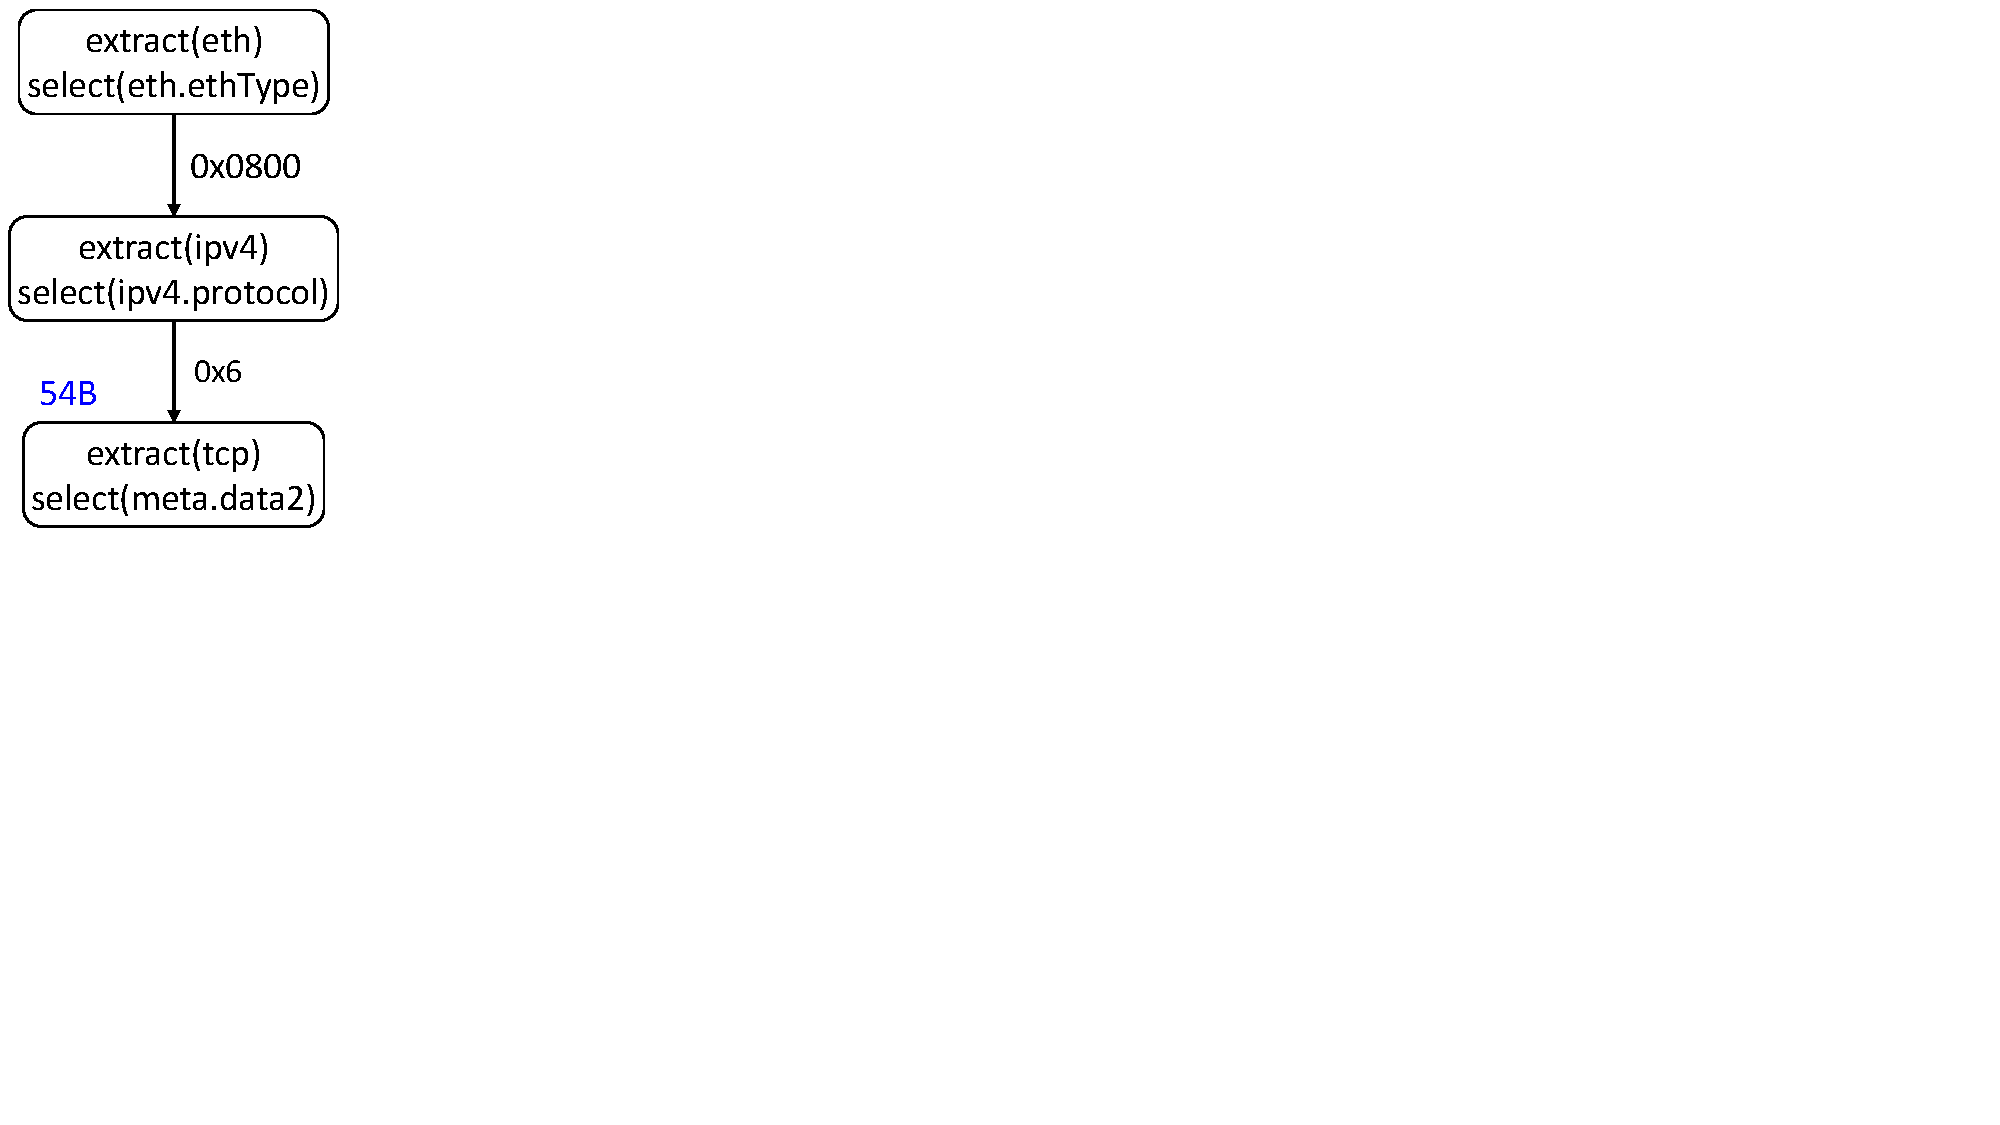
\includegraphics[trim=4 285 796 0, clip,scale=0.4]{parser-example-se-1}
        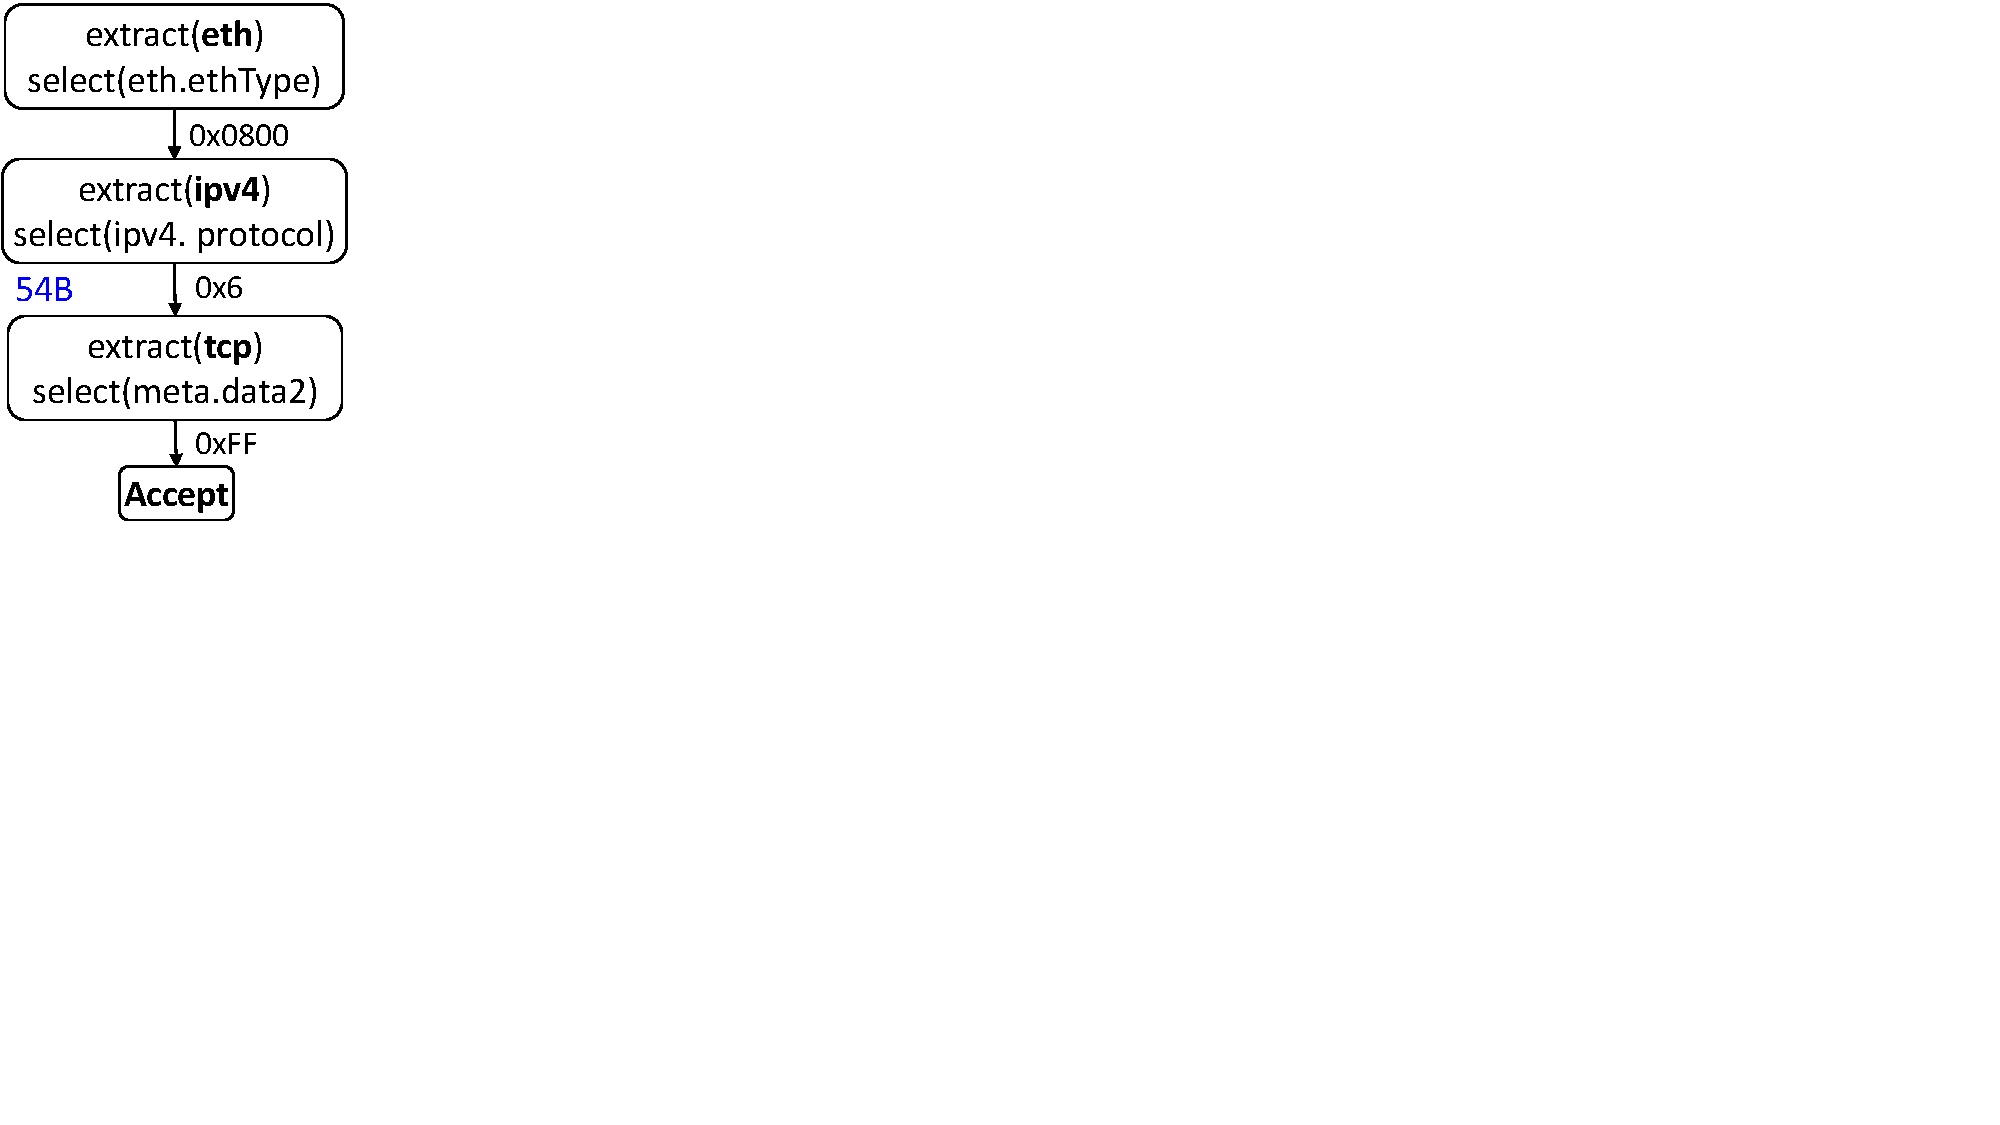
\includegraphics[trim=4 285 796 0, clip,scale=0.4]{parser-example-se-2}
        \caption{Parser Symbolic Execution}
        \label{subfig:parser-symbolic-execution}
    \end{subfigure}
    \begin{subfigure}[b]{.4\linewidth}
\begin{lstlisting}[frame=none]
control Pipe(inout hdr_t hdrs, out bit<16> nexthop_id, inout sm_t sm) {
  action process(bit<16> nh) {
    hdrs.ipv4.ttl = hdrs.ipv4 - 1;
    nexthop_id = nh;// setting out param
  }
  table ipv4_lpm_tbl {
    key = { hdrs.ipv4.dstAddr : lpm } 
    actions = { process; }
  }
  apply { ipv4_lpm_tbl.apply(); }
}
\end{lstlisting}
\caption{Match-Action Control Block}
\label{subfig:parser-symbolic-execution}
\end{subfigure}
\caption{Parser to Control Block Transformation}
\label{fig:parser-to-control-block-transformation}
\end{figure*}

For every parser state, we create a match key comprising key-fields from sets of keys. 
$(1)$ $visit$ variable assocociated with the set of all its ancestors and the state itself and
$(2)$ union of select expression of all of its evaluated instances.
In most cases, the union of select expression would have a single key-field, unless forward substitution has produced different expressions in the state's evaluated instances.

The \emph{start} being a special state has only one evaluated instance.
We create an action, called \emph{start\_action}, from the only instance of the start state.
Next, we visit parser states in topological order. 
We create match key for the current parser state as described above.
The match-key entries are created using keysetExpression and all possible paths represented to the state encoded using visit bit vector.
For each match key entry, we use appropriate action synthesised by next state's evaluated instance.

The apply body of the control block consists of an action call invalidating all the header instances, followed by the start\_action call and apply calls to the MATs created for parser states in topological order.



\subsubsection{Variable Length Headers and Loops Elimination}
\label{variable-length-headers-loops-and-elimination}
The two-argument extract method is replaced with a synthesised sub-parser with three arguments.
First to arguments are the same as two-argument extract method and the third arguments is maximum size of variable field.
The start state of the sub-parser contains a transition\-Statement with a select\-Expression.
The sub-parser contains a state for each possible value of variable field size that extracts constant number of bits using single argument extract method and transits to accept state.
The select\-Expression of the start state uses the variable field size parameter(the second parameter) to match on and transit to the corresponding next state.




\subsection{Deparser Block Transformation}
\label{subsection:deparser-block-transformation}
Recall that deparser blocks are specialized control blocks having packet\_out extern as one of the arguments.
The extern's emit method inserts bits on packets' bit-stream, if the header instance provided in the argument is valid, else no operation is performed.
We precisely perform the same operation on byte array buffer, but first we create a match-action table to push fixed number of bytes on the byte array buffer.
Recall that the program's parser transformation pops the total number of extracted bytes from the array buffer.
If the program's parser extracts less than $\mathcal{E}l$ for a particular packet, there are valid data on byte array.

The key of the table are created using valid bit of each header instance.
The table contains entries enumerating all possible combination of validity of the headers and action corresponding to each match key value to push the number of bytes equals to sum of lengths of all valid headers.


The deparser block may contain P4 language constructs like \emph{if-else} and \emph{switch} statements in addition of emit method call statements.
Therefore, deparser block may have multiple execution paths emitting the same header instances. 
We derive a directed-acyclic-graph, called \emph{emit graph}, with each node representing a emit call from the control flow graph of the deparser control block.
We synthesise a match-action table for every emit method call in deparser blocks.
Similar to one bit $visit$ variable for parser states, we create one bit variable, \emph{emit}, for each node in the emit graph.
The match key for the match-action table for an emit node comprises valid bit of the header instances passed as argument to its ancestors.
In addition, the match key includes $emit$ variables associated with the ancestors.
The idea behind introducing $emit$ variable is to record execution of previous emit calls in the control path and copy header instance  of emit call at appropriate location in the byte array buffer.



\subsection{(De)parser Control Block Optimization}
The transformation of parser and deparser blocks into match-action control blocks induces huge cost in terms of number of binary variables in data plane and multiple match-action tables.
Also, number of entries in the tables are of exponential order of binary variable fields in the tables.
In this section, we describe optimization methods to reduce per state match-action tables in transformed parser blocks into a single match-action table and eliminate all the binary variables.
 

\subsection{Real-Target Specific Transformation}

\subsubsection{Extracting Parallelism}
We extract the \emph{Packet-processing Schedule Graph} (PSG) of the micro-switch program to identify code and packet(data) parallelism.
A node represents an instance of either pkt\_in, logical buffers, pkt\-\_out, micro-switch program intrinsic metadata or collection of input or output arguments.
\begin{figure}[!h]
    \centering
    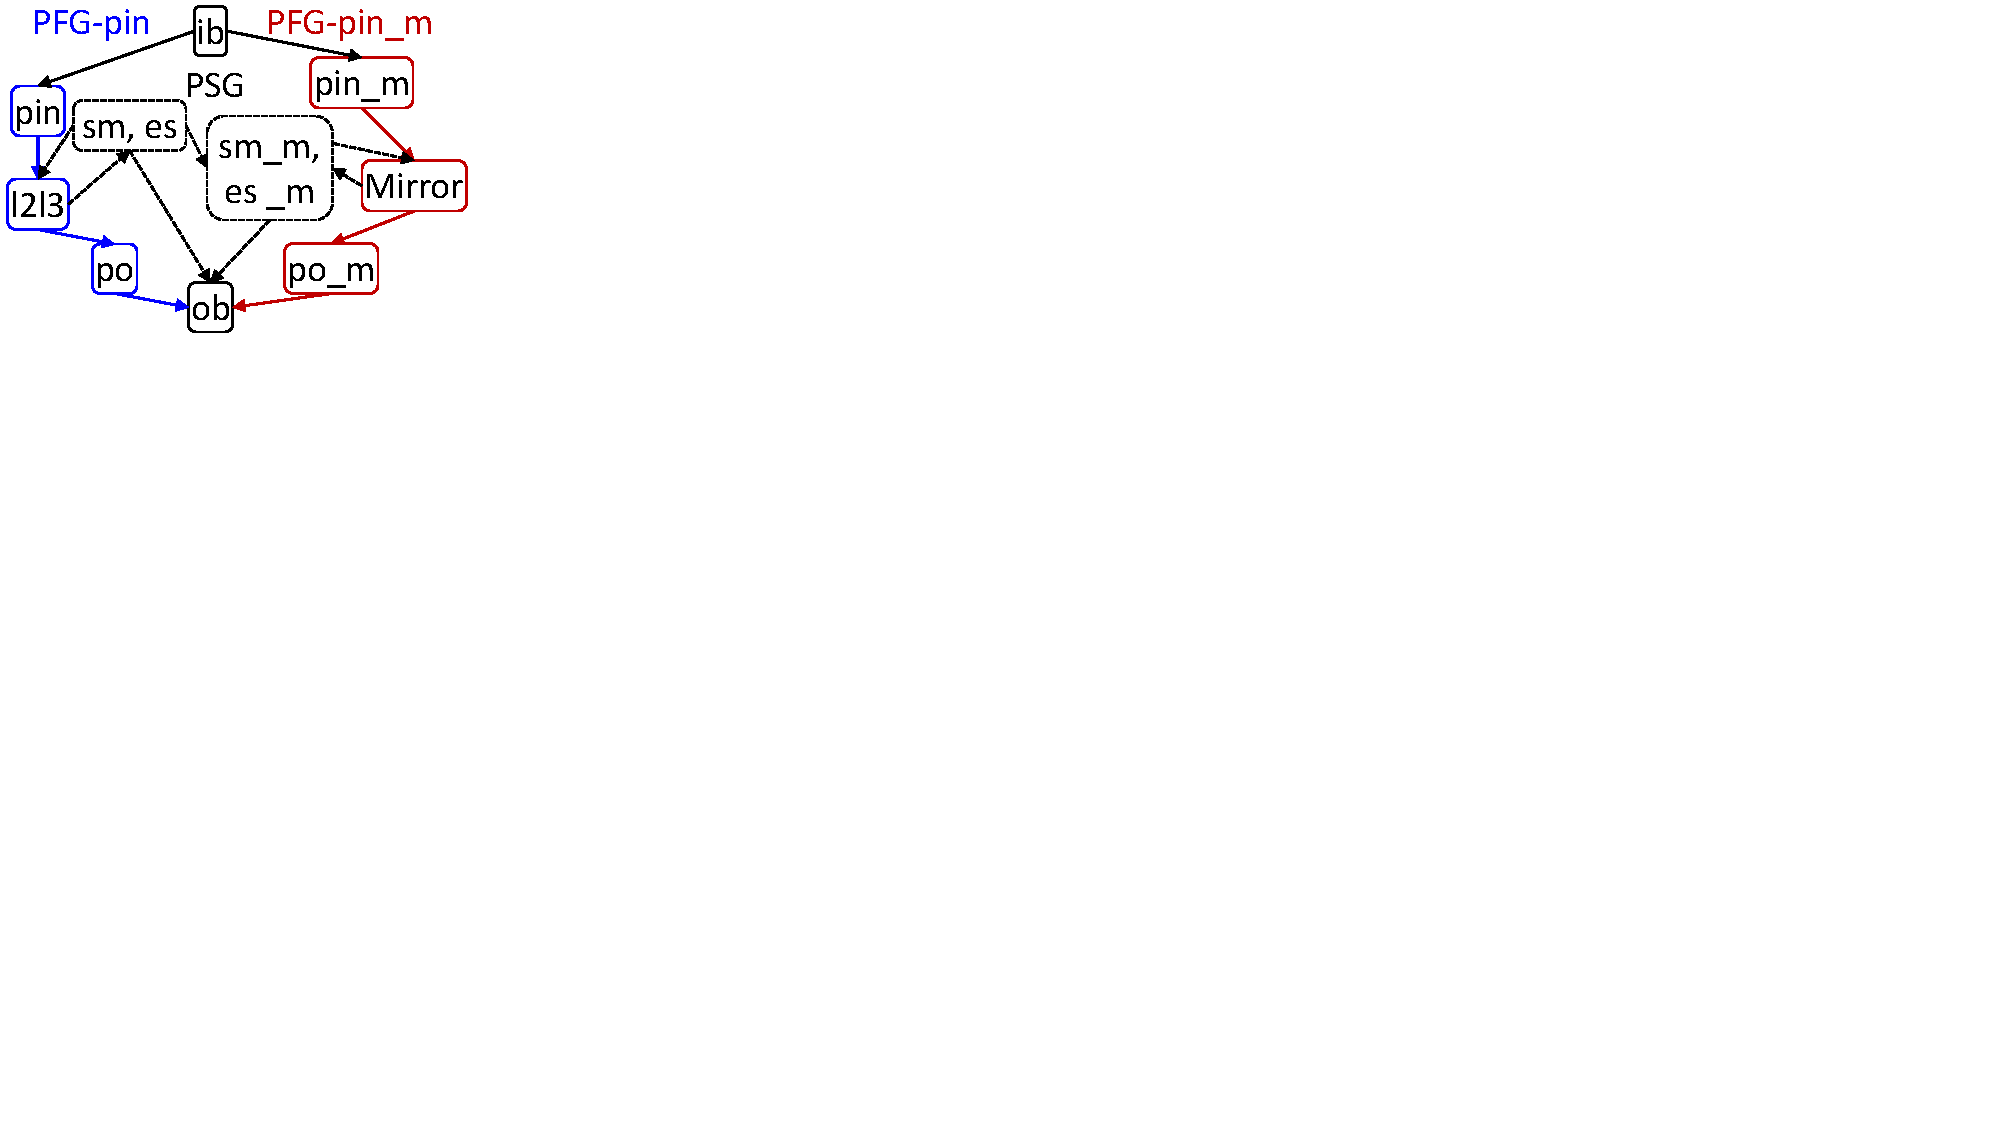
\includegraphics[trim=0 370 735 0, clip, scale=0.5]{psg}
    \caption{PSG for the \emph{rm} program (Figure \ref{fig:parallel-execution})}
    \label{fig:graph}
\end{figure}
The enqueue and dequeue method call are represented, respectively, by outgoing and incoming edges on the instances of packet\_in and packet\_out.
Every assignment statement is represented by a directed edge from the instance on the right to the left side.
To identify parallelism originating from packet duplication, we consider a subgraph of PSG, called packet flow graph (PFG).
PFG contains does not contain nodes representing instances of intrinsic metdata, input and output arguments.
The Figure \ref{fig:graph} shows the PFG and PSG of the micro-switch program shown in the Figure \ref{fig:parallel-execution}.
% If the program We remove in\_buf node and the edge represented by the dequeue operation.
The input(pkt\_in, params with \texttt{in} direction, in\_buf) arguments of the switch-program does not have any incoming edge.
We begin with computing dominator tree for the nodes representing the copies of pkt\_in input argument.
Next, we create a subgraph for each dominator tree containing nodes from the tree, incidence edges from the PFG.
If there is no path between nodes of any two subgraphs, the subgraphs represents code blocks that can should process copies the packet.
A path between nodes of subgraphs represents exchange of metadata between code blocks processing copies the same packet.
It can be facilitated based on capability of target devices.
If there is a loop in the PFG, compilation fails.

We briefly explain mechanism to realise parallel processing using v1model architecture for the scenario.
We synthesize a metadata variable to track cloned copies. 
The variable is updated after the execution of parallel code block.
The code block is encapsulated in an \emph{if} statement. 
It is executed only if the metadata variable matches with a constant value assigned for its execution.


\subsubsection{Control Block Constraints}
$\mu$SA pipelines contain single programmable control block. 
It provides intrinsic metadata as logical externs (es\_t) and a structure (sm\_t) to use in the control block.
We map $\mu$SA-specific intrinsic metadata to the ones defined in architectures of real targets.
We partition the CFG of $\mu$SA pipelines' programmable block into multiple CFGs to enforce accessibility constraints of target's intrinsic metadata in its control block.

Let's consider v1model architecture of simple\_switch target device for an example.
A two-state finite-state machine is used to capture ingress and egress pipeline blocks'  accessibility constraint on egress port and queueing metadata.
Each state represents extra conditions to visit CFG nodes in topological order.
State transition occurs when the graph traversal can not be continued due to absence of nodes without incoming edges.
In the first state, the graph traversal does not visit nodes representing multicast\_engine's apply or egress\_spec's get\_egress\_port or get\_value methods call statements.
When the traversal can not progress any further, we create partitions of visited and non-visited nodes.
In the second state, we do not visit nodes representing egress\_spec's get\_egress\_port methods call statements.


There can be multiple edges representing control branches between the partitions.
We synthesise \emph{partition} metadata that is assigned a unique value for each control branch in the first partition.
The second partition uses the metadata and if condition to resume execution on appropriate control branch.
Also, partitioned code may access the same local declaration variables.
These shared local variables along with the \emph{partition} metadata are passed as user-defined metadata between ingress and egress control block.
We insert recirculate method call at the end of even numbered partitions.


\section*{Acknowledgments}

\bibliographystyle{abbrv} 
\begin{small}
\bibliography{main}
\end{small}

\end{document}

